%*******************************************************************************
%****************************** Sixth Chapter *********************************
%*******************************************************************************

\chapter{Characterisation of III-Nitride Microrods}

\section[Background]{Background}
The growth of GaN nano- and micro-rods provides an attractive solution for the mitigation of various material issues which plague hetero-epitaxially grown III-nitrides, as discussed in section \ref{nwsectionintro}. Threading dislocations (TDs) in III-nitride rods have been shown to bend toward the sidewall facets in free-standing rods rather than threading through the entire rod, resulting in a  defect-free region of the rod \cite{Bergbauer2010,Tessarek2013}. Furthermore, the large surface-to-bulk-volume ratio of free-standing rods results in effective lateral strain relaxation \cite{Zhao2015}, allowing for a reduction in the piezoelectric polarization fields in III-nitrides. As a result of these potential benefits, many nanorod based optoelectronic devices have been demonstrated, ranging from lasers to single photon sources, as discussed in greater detail in section \ref{nwsectionintro}.
This section will introduce the work done in characterising the effect of different growth conditions on the structural and optical properties of MOVPE grown III-nitride microrods.

\subsection{Nanorod Growth}
\label{nanorod growth}
The growth of III-nitride micro- and nanorods remains an active area of research, due to the plethora of methods available and the large range of potential applications requiring rods of different sizes, densities and with varying structural and compositional properties. 
Top-down methods for the production of rods involving lithography-related synthesis have been widely investigated. This approach is shown schematically in Fig.\ref{topdown}. Approaches such as photon \cite{Liu201558} and electron beam lithography \cite{Maliakkal2015}, plasma and wet etching \cite{Debnath2014}  and FIB micro-machining \cite{Dhara2010} which enable the production of site-controlled, uniform rods have been reported. However, these methods intrinsically produce surface damage in the rods and are limited by the resolution of the patterning techniques \cite{Bao2016}.
\begin{figure}[h]
	\centering
	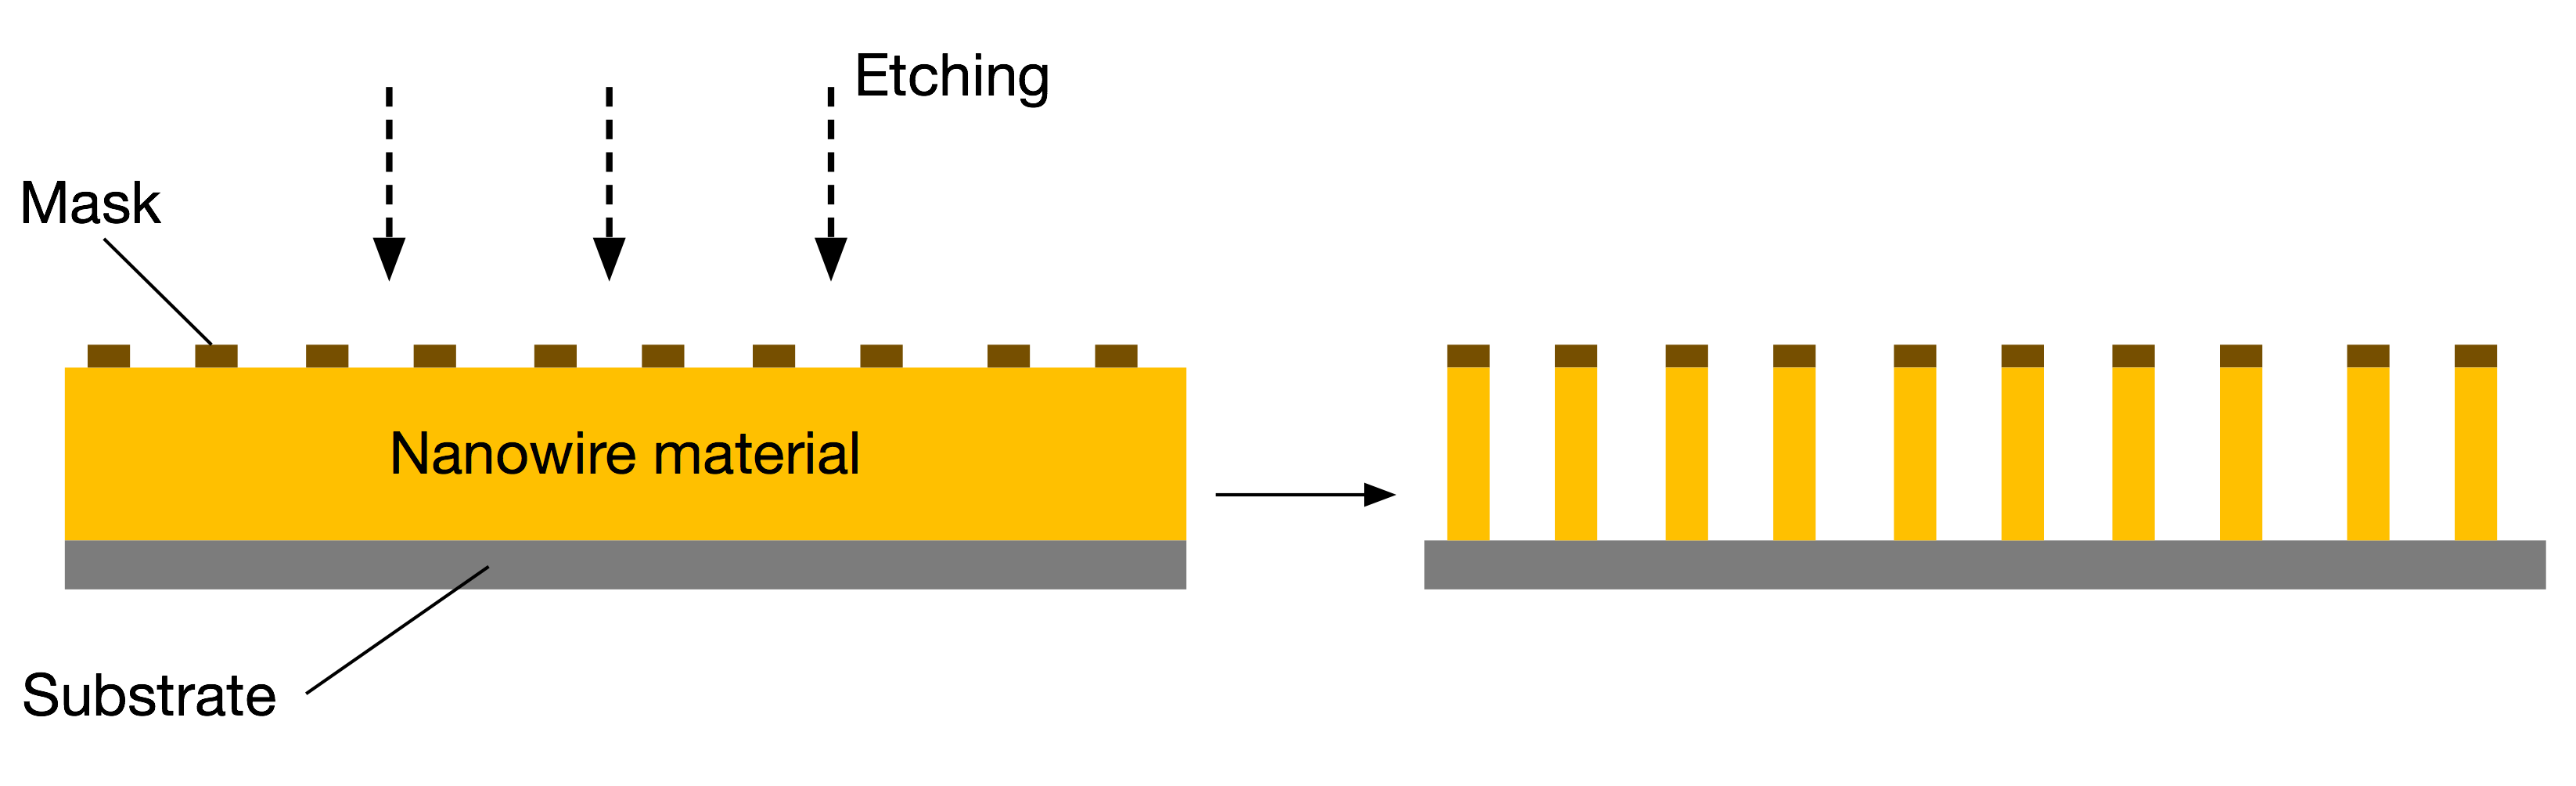
\includegraphics[width=1\textwidth]{Figs/Ch6/topdown.png}
	\caption {Top-down approach to nanorod fabrication. The mask is not required if a site-specific etching method such as electron beam lithography or FIB micromachining is used. Reproduced from \cite{Bao2016}}
	\label{topdown}
\end{figure}
\FloatBarrier 
Bottom-up methods are thus preferred in applications where surface damage can hinder device performance. In this context we will discuss nanowire epitaxy, although processes such as oxide-assisted laser ablation of GaN may also be used for the production of nanowires where no directional or positional control is required \cite{Shi2001}. In the case of catalyst induced epitaxy, Au \cite{Hou2011}, Fe \cite{Duan2000}, Ni \cite{Cheze2010} or La \cite{Chen2010} catalytic particles can be used in an N-rich environment to grow nanorods epitaxially. In these cases, the growth rate of the rods is determined by the availability of group III atoms, which accumulate in the extrinsic metal particles \cite{Geelhaar2007}. Vapour-liquid-solid  \nomenclature[z-VLS]{VLS}{Vapour-Liquid-Solid} (VLS) growth is the primary mechanism for the catalyst-induced growth of rods. The VLS process can be considered as a three phase system with the supply, collector and crystal in the vapour, liquid and solid phase respectively. The three phase boundary \nomenclature[z-TPB]{TPB}{Three Phase Boundary} (TPB) is the perimeter of the growth front in the nanorod \cite{Chen2015}. During the growth process the semiconductor material is incorporated into the nanorod through the vapour-liquid interface due to the metallic particle. The further addition of semiconductor source material results in the precipitation of the material, resulting in the liquid/solid interface often known as the growth interface.This is shown schematically in Fig.\ref{VLS}. Catalyst-induced growth provides excellent control of the rod dimensions as the diameter of the rods is determined by the size of the catalytic particles, however these particles remain on top of the rods after the growth is completed.
\begin{figure}[h]
	\centering
	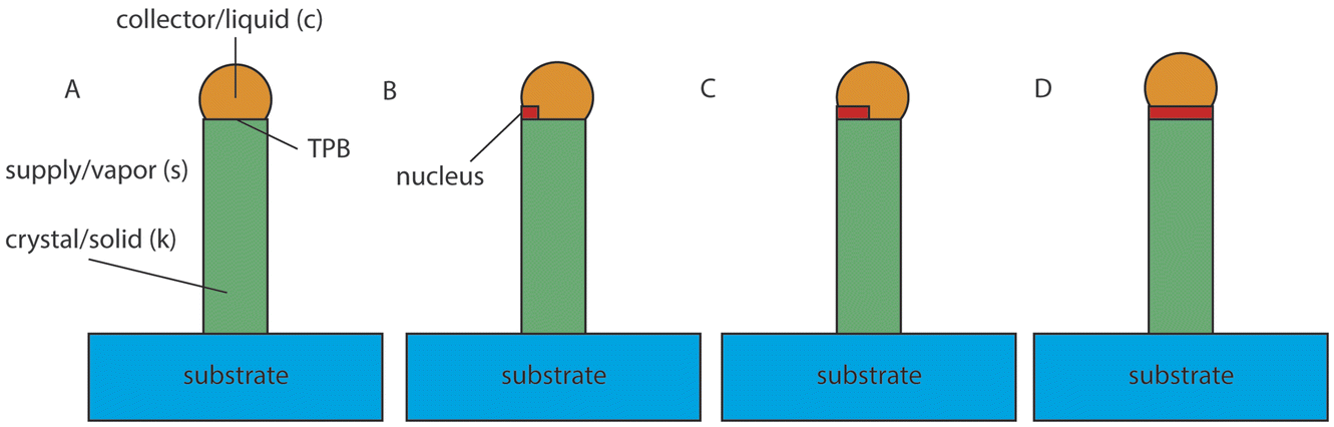
\includegraphics[width=1\textwidth]{Figs/Ch6/VLS}
	\caption {Catalyst induced nanowire growth mechanism. Reproduced from \cite{Chen2015}.}
	\label{VLS}
\end{figure}
\FloatBarrier

In order to avoid issues which may arise due to the use of catalytic particles, extrinsic particle free epitaxy may be used. Such methods involve either direct epitaxy \cite{Cheze2010} or selective area epitaxy \cite{Hersee2006}. In the case of direct epitaxy, the nanowires are obtained in specific growth conditions chosen to enhance vertical growth and restrict lateral growth of III-nitride layers thus producing rods. Selective area epitaxy involves a substrate patterning step prior to growth in order to induce rod growth. It has been suggested that the growth of III-nitride rods by extrinsic particle free epitaxy MOVPE requires a V/III ratio below 200 and hydrogen carrier gas \cite{Tessarek2014a}. These conditions promote vertical growth in the \textit{c}-direction with \textit{m}-plane facets for N-polar GaN due to the passivating effect of the hydrogen on the nitrogen atoms on the surface of the crystal \cite{Li2011}. The vertical growth of undoped rods is however generally limited to aspect ratios below 1 \cite{Tessarek2014a}. Si, typically used as an \textit{n}-type dopant, has been shown to induce vertical growth, resulting in aspect ratios exceeding 100 \cite{Tessarek2013,Koester2010}.
 
\section{Experimental}
In this section we will describe the work done by the author in characterising microrods grown at the Cambridge Centre for Gallium Nitride by Dr. Tongtong Zhu.

\subsection{Microrod Growth}

The microrod samples were grown by MOVPE in a 6 x 2 in. Thomas Swan close-coupled showerhead reactor on 2 inch \textit{c}-plane sapphire substrates using trimethylgallium, trimethylindium, and ammonia as precursors and silane as source of silicon. After annealing the sapphire substrate at \SI{1050}{\degree}C for 10 mins in a $\mathrm{H_{2}}$ atmosphere, a low temperature GaN nucleation layer of thickness 5 nm was deposited at \SI{550}{\degree}C and annealed in $\mathrm{H_{2}}$ at \SI{1000}{\degree}C for 3 mins to serve as a seed layer for the subsequent microrod growth. The GaN microrods were then grown at \SI{995}{\degree}C  using $\mathrm{H_{2}}$ as the carrier gas and a V/III ratio of 50. Two samples were grown in order to demonstrate the effect of Si on the structural and optical properties of core-shell InGaN/GaN microrods. For sample A (C6364A), the GaN microrod was grown using a reactor pressure of 300 Torr, and a constant silane flow of 0.2 µmol/min was supplied throughout for 720 s to enhance the vertical growth rate. Sample B (C6525A) was grown at a reactor pressure of 500 Torr. A similar silane flow was supplied only for 120 s to initiate the vertical growth. The silane flow was then ramped down to 0.02 µmol/min in 60 seconds and continued for another 240 s for the nanorod growth. After the GaN microrod growth, five-period core-shell InGaN/GaN multiple quantum wells were grown  under identical conditions for both samples with a V/III ratio of 5000 at 300 Torr and using $\mathrm{N_{2}}$ as the carrier gas. The InGaN QWs were grown at \SI{730}{\degree}C and the GaN barriers were grown at \SI{885}{\degree}C.

\subsection{Microrod Emissive Properties}
\label{rod emission}
Microrods from sample A are shown in Fig.\ref{Asub}. We can see from the panchromatic CL image shown in Fig.\ref{Asub}.b that only the top 1 $\mathrm{\mu}$m of the rods is brightly emitting.

\begin{figure}[th]
	%\hspace*{-2cm}
	\begin{subfigure}[b]{0.4\textwidth}
		\centering
		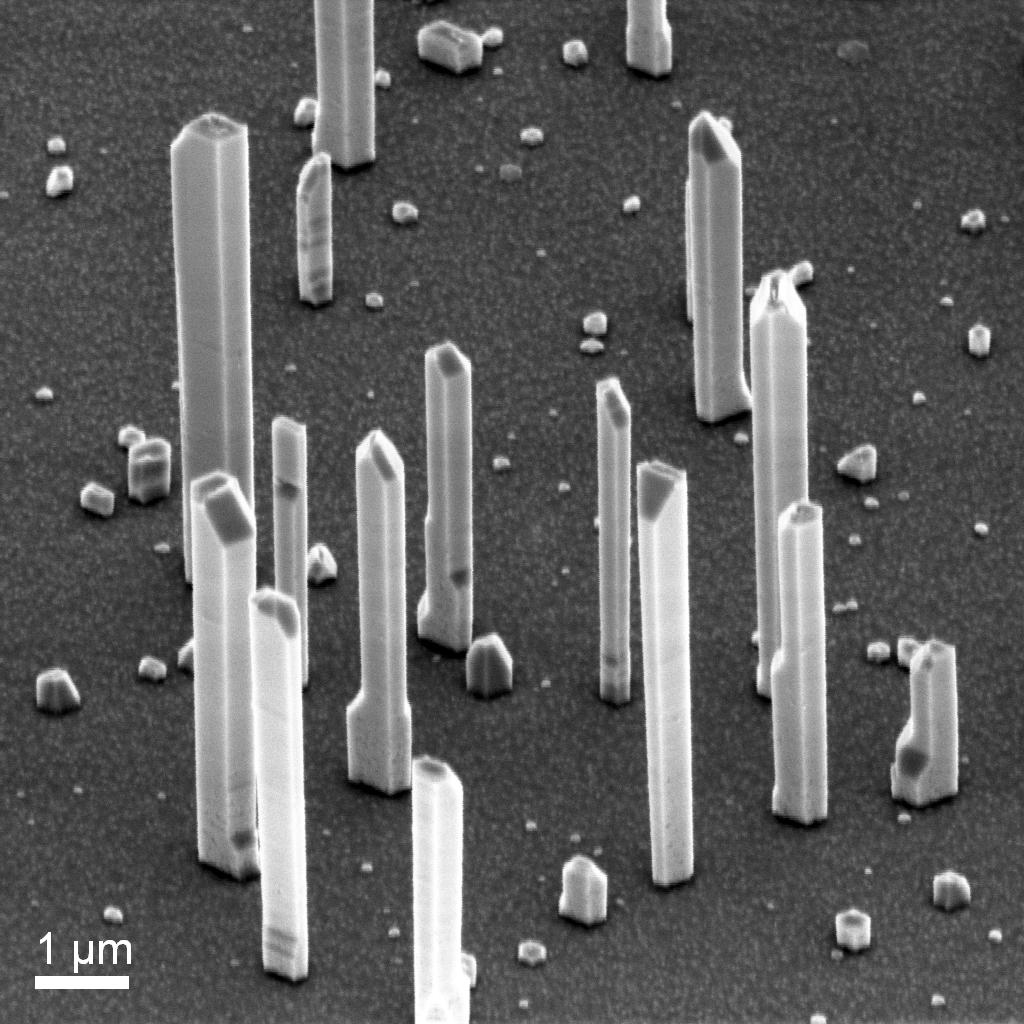
\includegraphics[width=1\linewidth]{Figs/Ch6/SEM_7262_2}
		\caption{}
		
	\end{subfigure}%
	\hspace*{1.5cm}
	\begin{subfigure}[b]{0.4\textwidth}
		\centering
		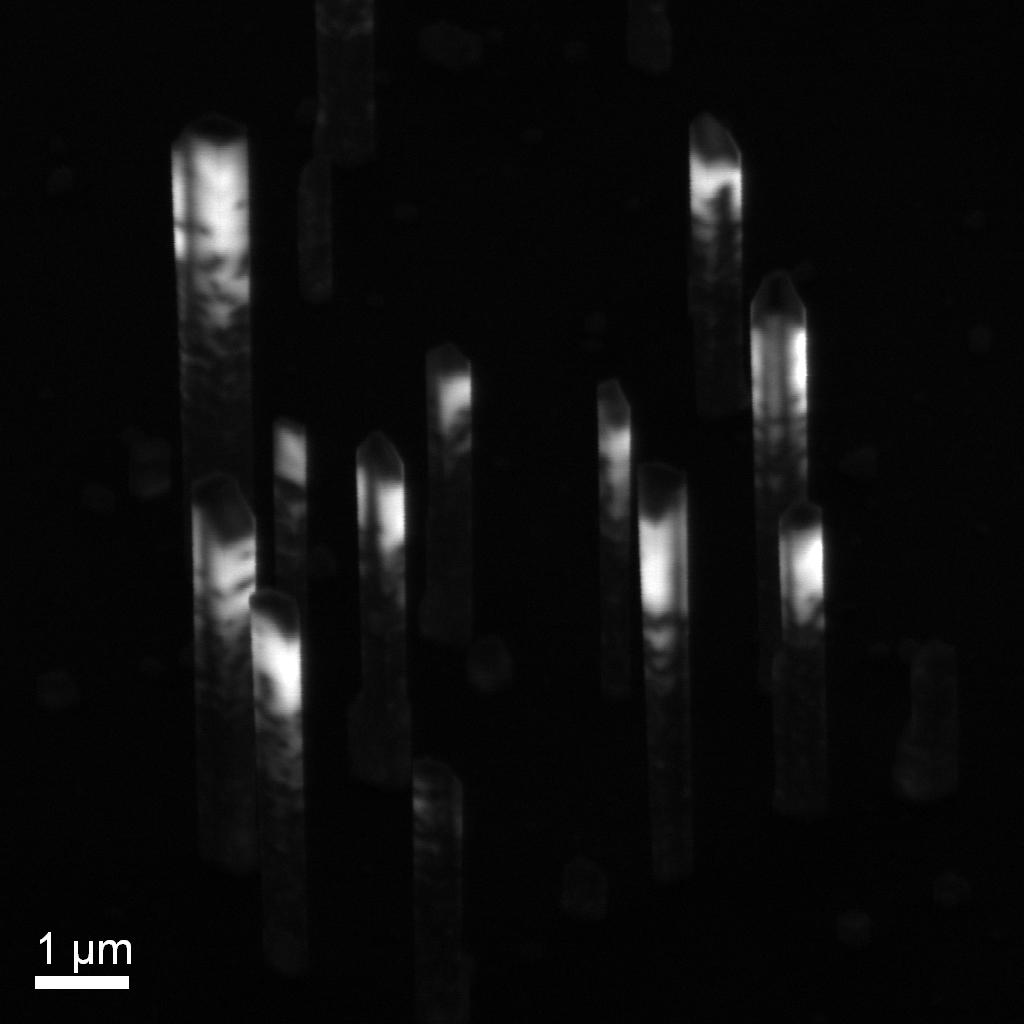
\includegraphics[width=1\linewidth]{Figs/Ch6/CL_7262_2}
		\caption{}
	\end{subfigure}%
	
	\caption{a) SEM micrograph and b) panchromatic CL image at 5 kV of microrods from sample A. Images courtesy of Dr. Tongtong Zhu.}
	\label{Asub}
\end{figure}
\FloatBarrier

Microrods from sample B are shown in Fig.\ref{Bsub}. In contrast to the rods shown in Fig.\ref{Asub}, rods from the sample B show relatively uniform emission in the panchromatic CL, though some dark regions are observable at the base of some rods.

\begin{figure}[th]
	%\hspace*{-2cm}
	\begin{subfigure}[b]{0.4\textwidth}
		\centering
		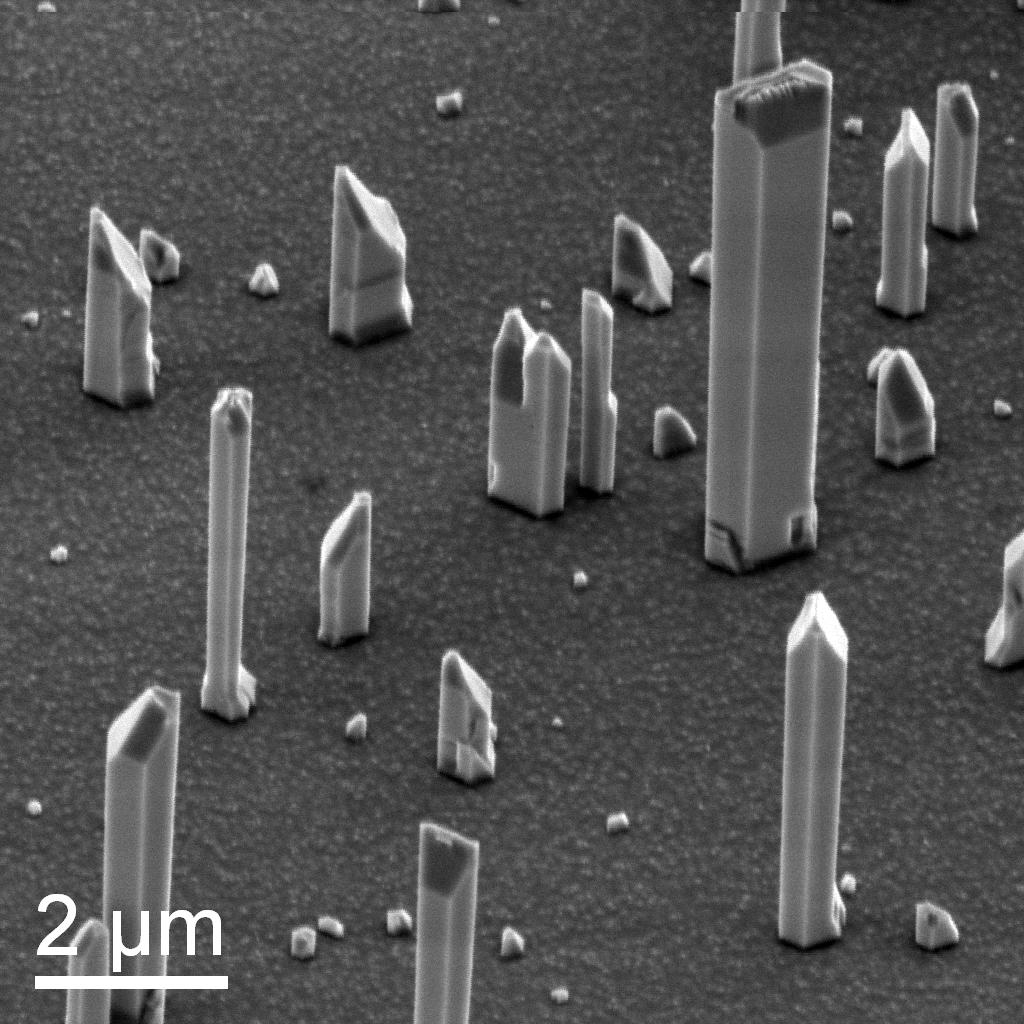
\includegraphics[width=1\linewidth]{Figs/Ch6/SEM_7481x}
		\caption{}
		
	\end{subfigure}%
	\hspace*{1.5cm}
	\begin{subfigure}[b]{0.4\textwidth}
		\centering
		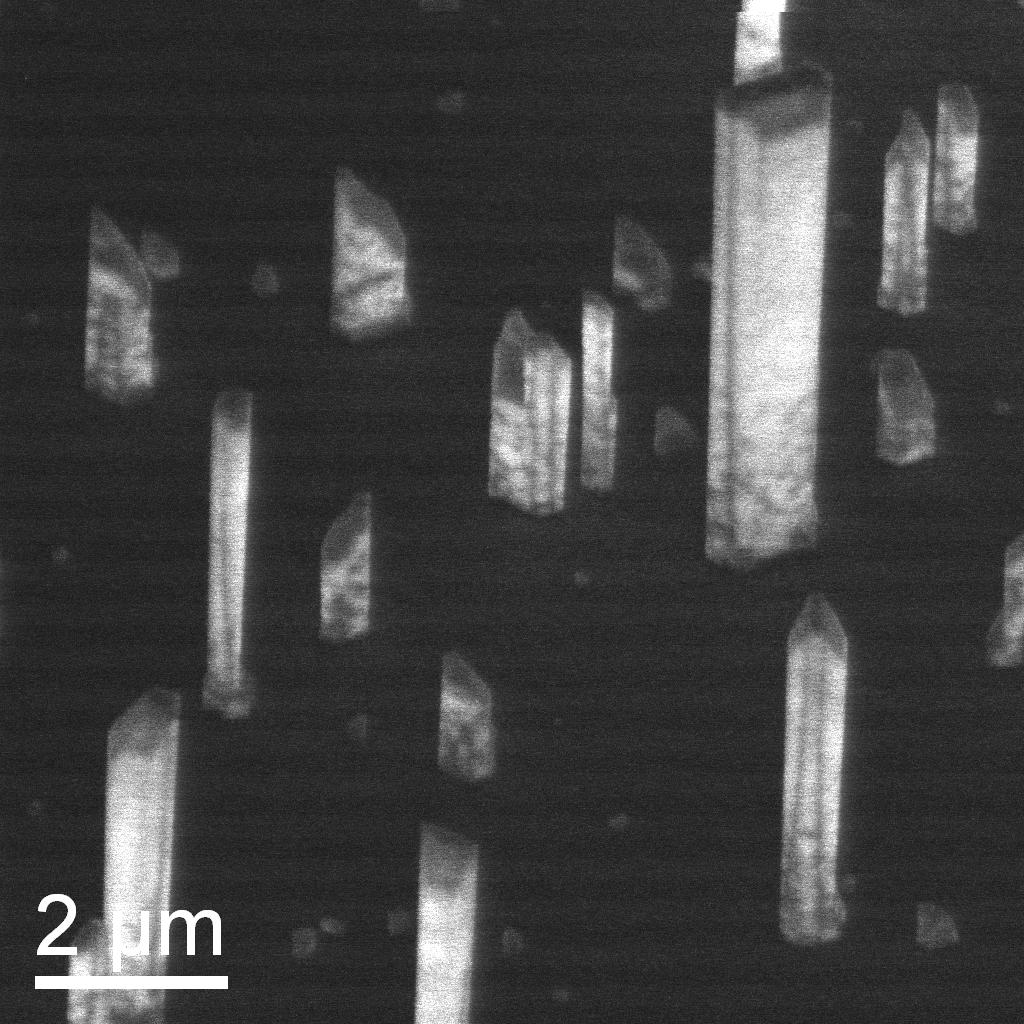
\includegraphics[width=1\linewidth]{Figs/Ch6/CL_7481x}
		\caption{}
	\end{subfigure}%
	
	\caption{a) SEM micrograph and b) panchromatic CL image at 5kV of microrods from sample B. Images courtesy of Dr. Tongtong Zhu.}
	\label{Bsub}
\end{figure}
\FloatBarrier

Microrods from both samples were harvested and dispersed on a silicon substrate for correlated optical and structural analysis. A representative rod harvested from sample A is shown in Fig.\ref{sampleAscan}. A CL linescan was taken through the centre of the rod and is shown in Fig.\ref{sampleAscanCL}. The linescan was taken over approximately 6  $\mathrm{\mu}$m (corresponding to the length of the rod) at a step size of 10 nm with a dwell time of 0.5s per acquisition.

\begin{figure}[!h]
	\centering
	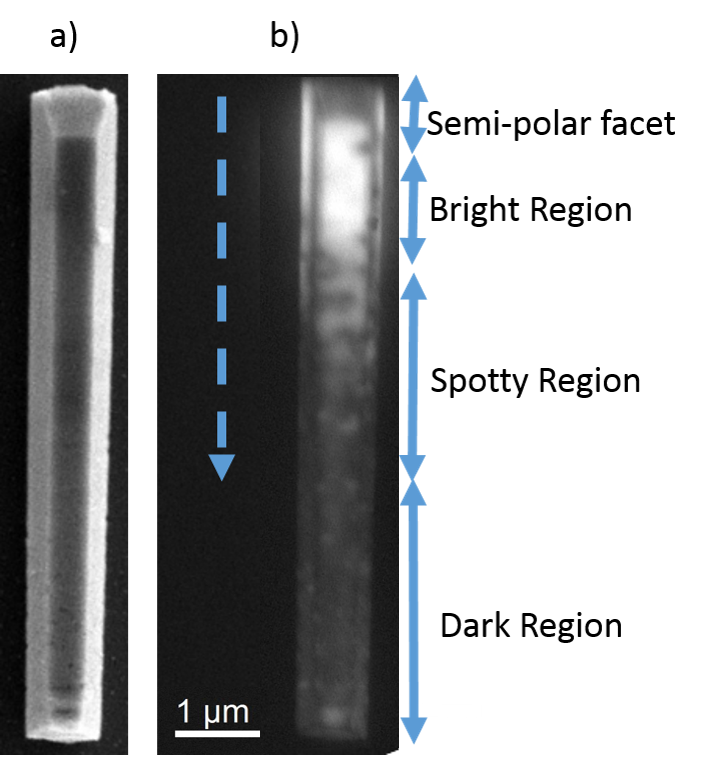
\includegraphics[width=0.48\textwidth]{Figs/Ch6/A-CL-scan.png}
	\caption {a) SEM image and b) panchromatic CL for a rod harvested from sample A on a silicon substrate. Different regions of the rod which are apparent in the panchromatic CL are labelled.}
	\label{sampleAscan}
\end{figure}
\FloatBarrier

\begin{figure}[!h]
	\centering
	\includegraphics[width=1\textwidth]{Figs/Ch6/CLscan}
	\caption {CL linescan taken at 10 nm steps along a rod from sample A denoted by the dashed blue arrow in Fig.\ref{sampleAscan}.}
	\label{sampleAscanCL}
\end{figure}
\FloatBarrier

Moving from the top to the bottom of the rod the trend shown by Fig.\ref{sampleAscanCL} is clear: the CL emission eventually vanishes.
Sample CL spectra taken from different regions of the rod are shown below in Fig.\ref{A-spectra}, with their respective normalisation factors. It appears that emission from the darker portion of the rod with a peak at 448 nm is greatly redshifted relative to the upper regions which shows peak CL emission around 410 nm.

\begin{figure}[!th]
	%\hspace*{-2cm}
	\begin{subfigure}[b]{0.35\textwidth}
		\centering
		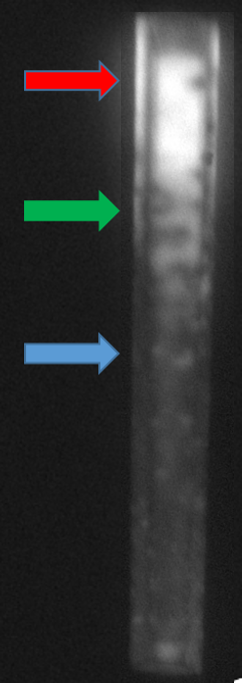
\includegraphics[width=0.5\linewidth]{Figs/Ch6/CL-linescanloc}
		\caption{}
		
	\end{subfigure}%
	\hspace*{-1cm}
	\begin{subfigure}[b]{0.6\textwidth}
		\centering
		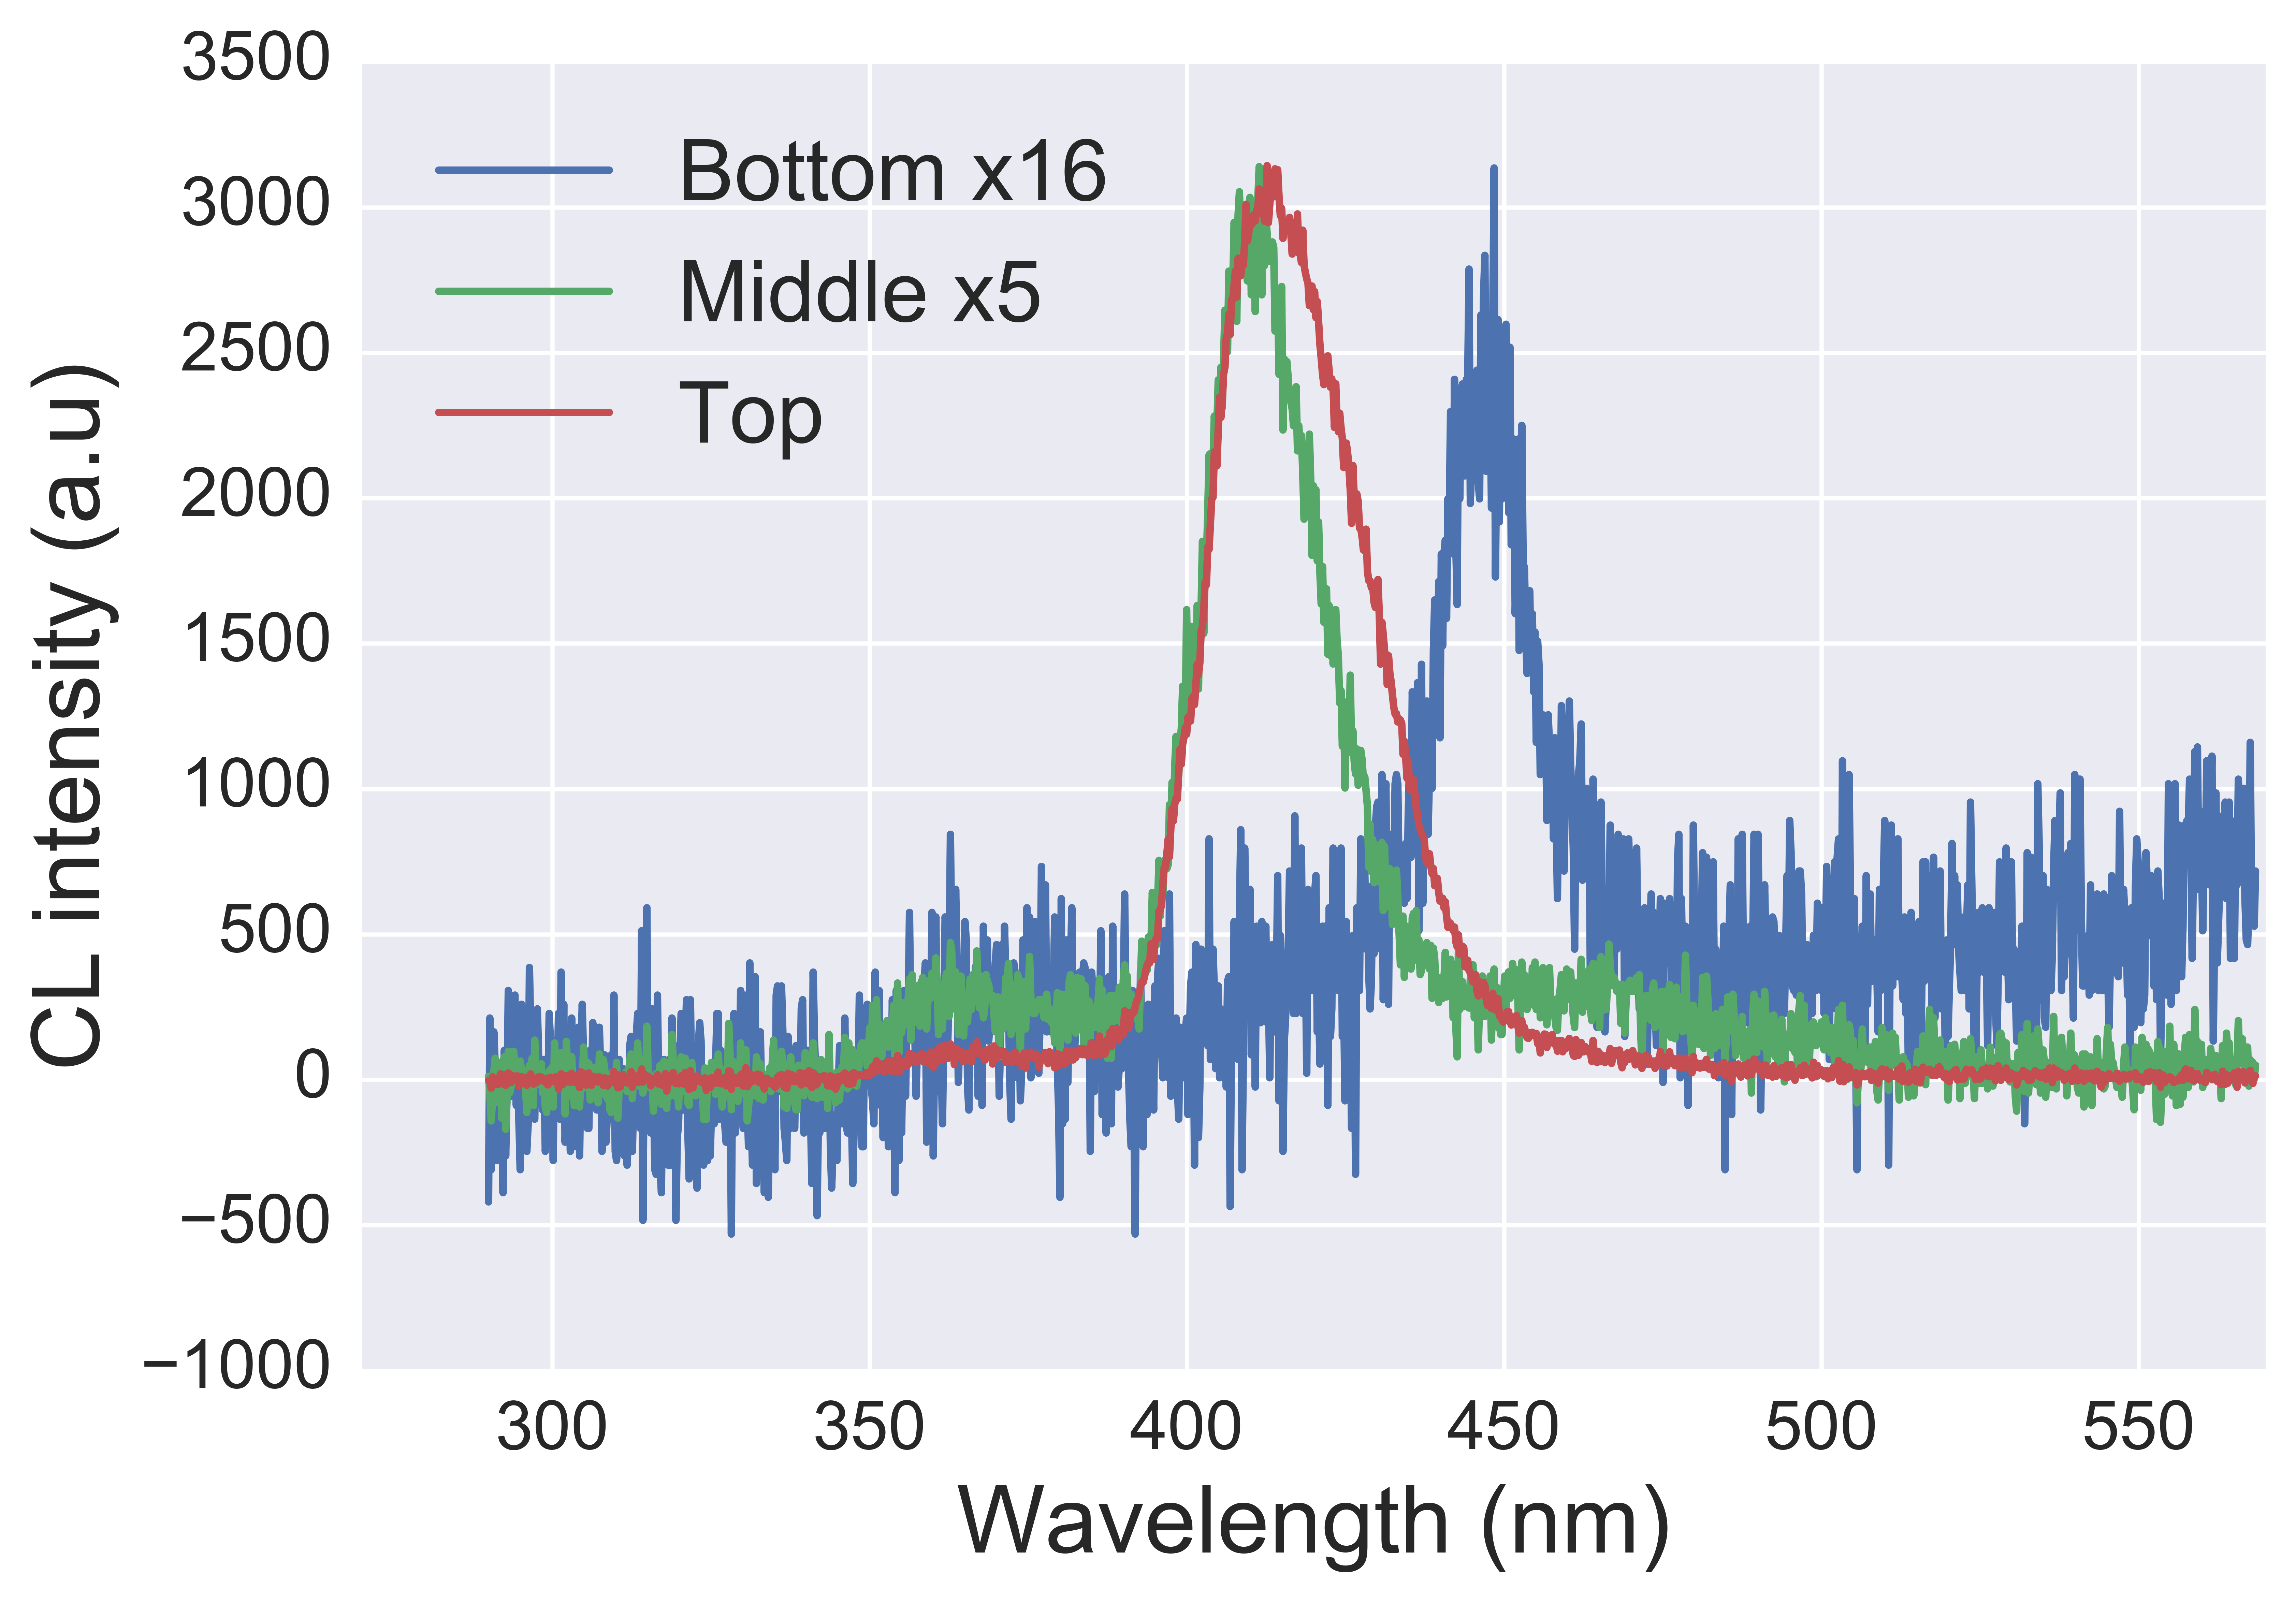
\includegraphics[width=1\linewidth]{Figs/Ch6/C6364}
		\caption{}
	\end{subfigure}%
	
	\caption{a) Panchromatic CL image showing the locations at which the CL spectra were taken b) CL spectra taken from the top, middle and bottom of the linescan with the respective normalisation factors shown in the legend.}
	\label{A-spectra}
\end{figure}
\FloatBarrier

The same experiment was repeated with rods harvested from sample B. These microrods exhibited far more homogeneous emission, as evidenced by the panchromatic CL image shown in Fig.\ref{sampleBscan}.b. 
\begin{figure}[!ht]
	\centering
	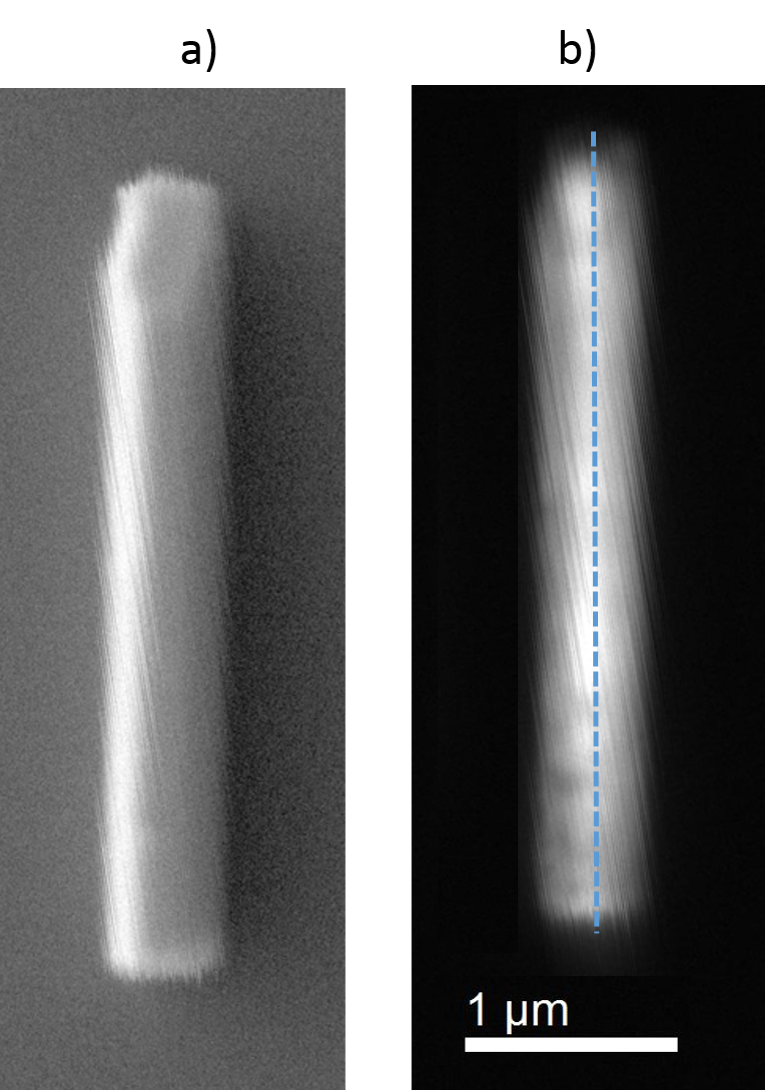
\includegraphics[width=0.28\textwidth]{Figs/Ch6/B-2CL-scan.png}
	\caption {a) SEM image and b) panchromatic CL for a rod harvested from sample B on a silicon substrate. The dashed blue line shows the location of the CL line scan.}
	\label{sampleBscan}
\end{figure}
\FloatBarrier

A line scan along the entire length of the brightly emitting rod was taken with a step size of 14 nm and a dwell time of 0.5 s per acquisition, the location of the linescan is denoted by the dashed blue line in Fig.\ref{sampleBscan}.b. The linescan data is shown in Fig.\ref{sampleBscanCL}. We can observe that although there is a slight shfiting of the peak CL wavelength and a reduction in the CL linewidth along the length of the microrod, the peak intensity remains relatively constant from the top to the bottom when compared with the microrod harvested from sample A.

\begin{figure}[!h]
	\centering
	\includegraphics[width=1\textwidth]{Figs/Ch6/CLscan1}
	\caption{CL line scan denoted by the dashed blue arrow in Fig.\ref{sampleBscan}.}
	\label{sampleBscanCL}
\end{figure}
\FloatBarrier

Non-normalised Individual CL spectra taken from the top, middle and bottom regions of the rod are shown in Fig.\ref{B-spectra}.b. We can observe that the peak CL intensities observed along the rod are generally consistent from the top to the bottom of this microrod when compared to the results from microrod A.We note the peak CL wavelength shifts from 420 nm to 408 nm moving from the top to the bottom of the rod, an effect which can also be seen in Fig.\ref{sampleBscanCL}.

\begin{figure}[!th]
	%\hspace*{-2cm}
	\begin{subfigure}[!th]{0.3\textwidth}
		\centering
		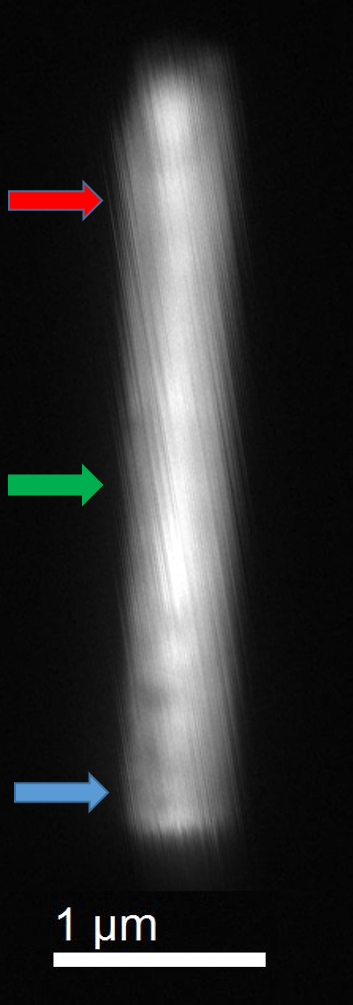
\includegraphics[width=0.5\linewidth]{Figs/Ch6/CL-linescanloc2}
		\caption{}
		
	\end{subfigure}%
	\hspace*{-1cm}
	\begin{subfigure}[!th]{0.6\textwidth}
		\centering
		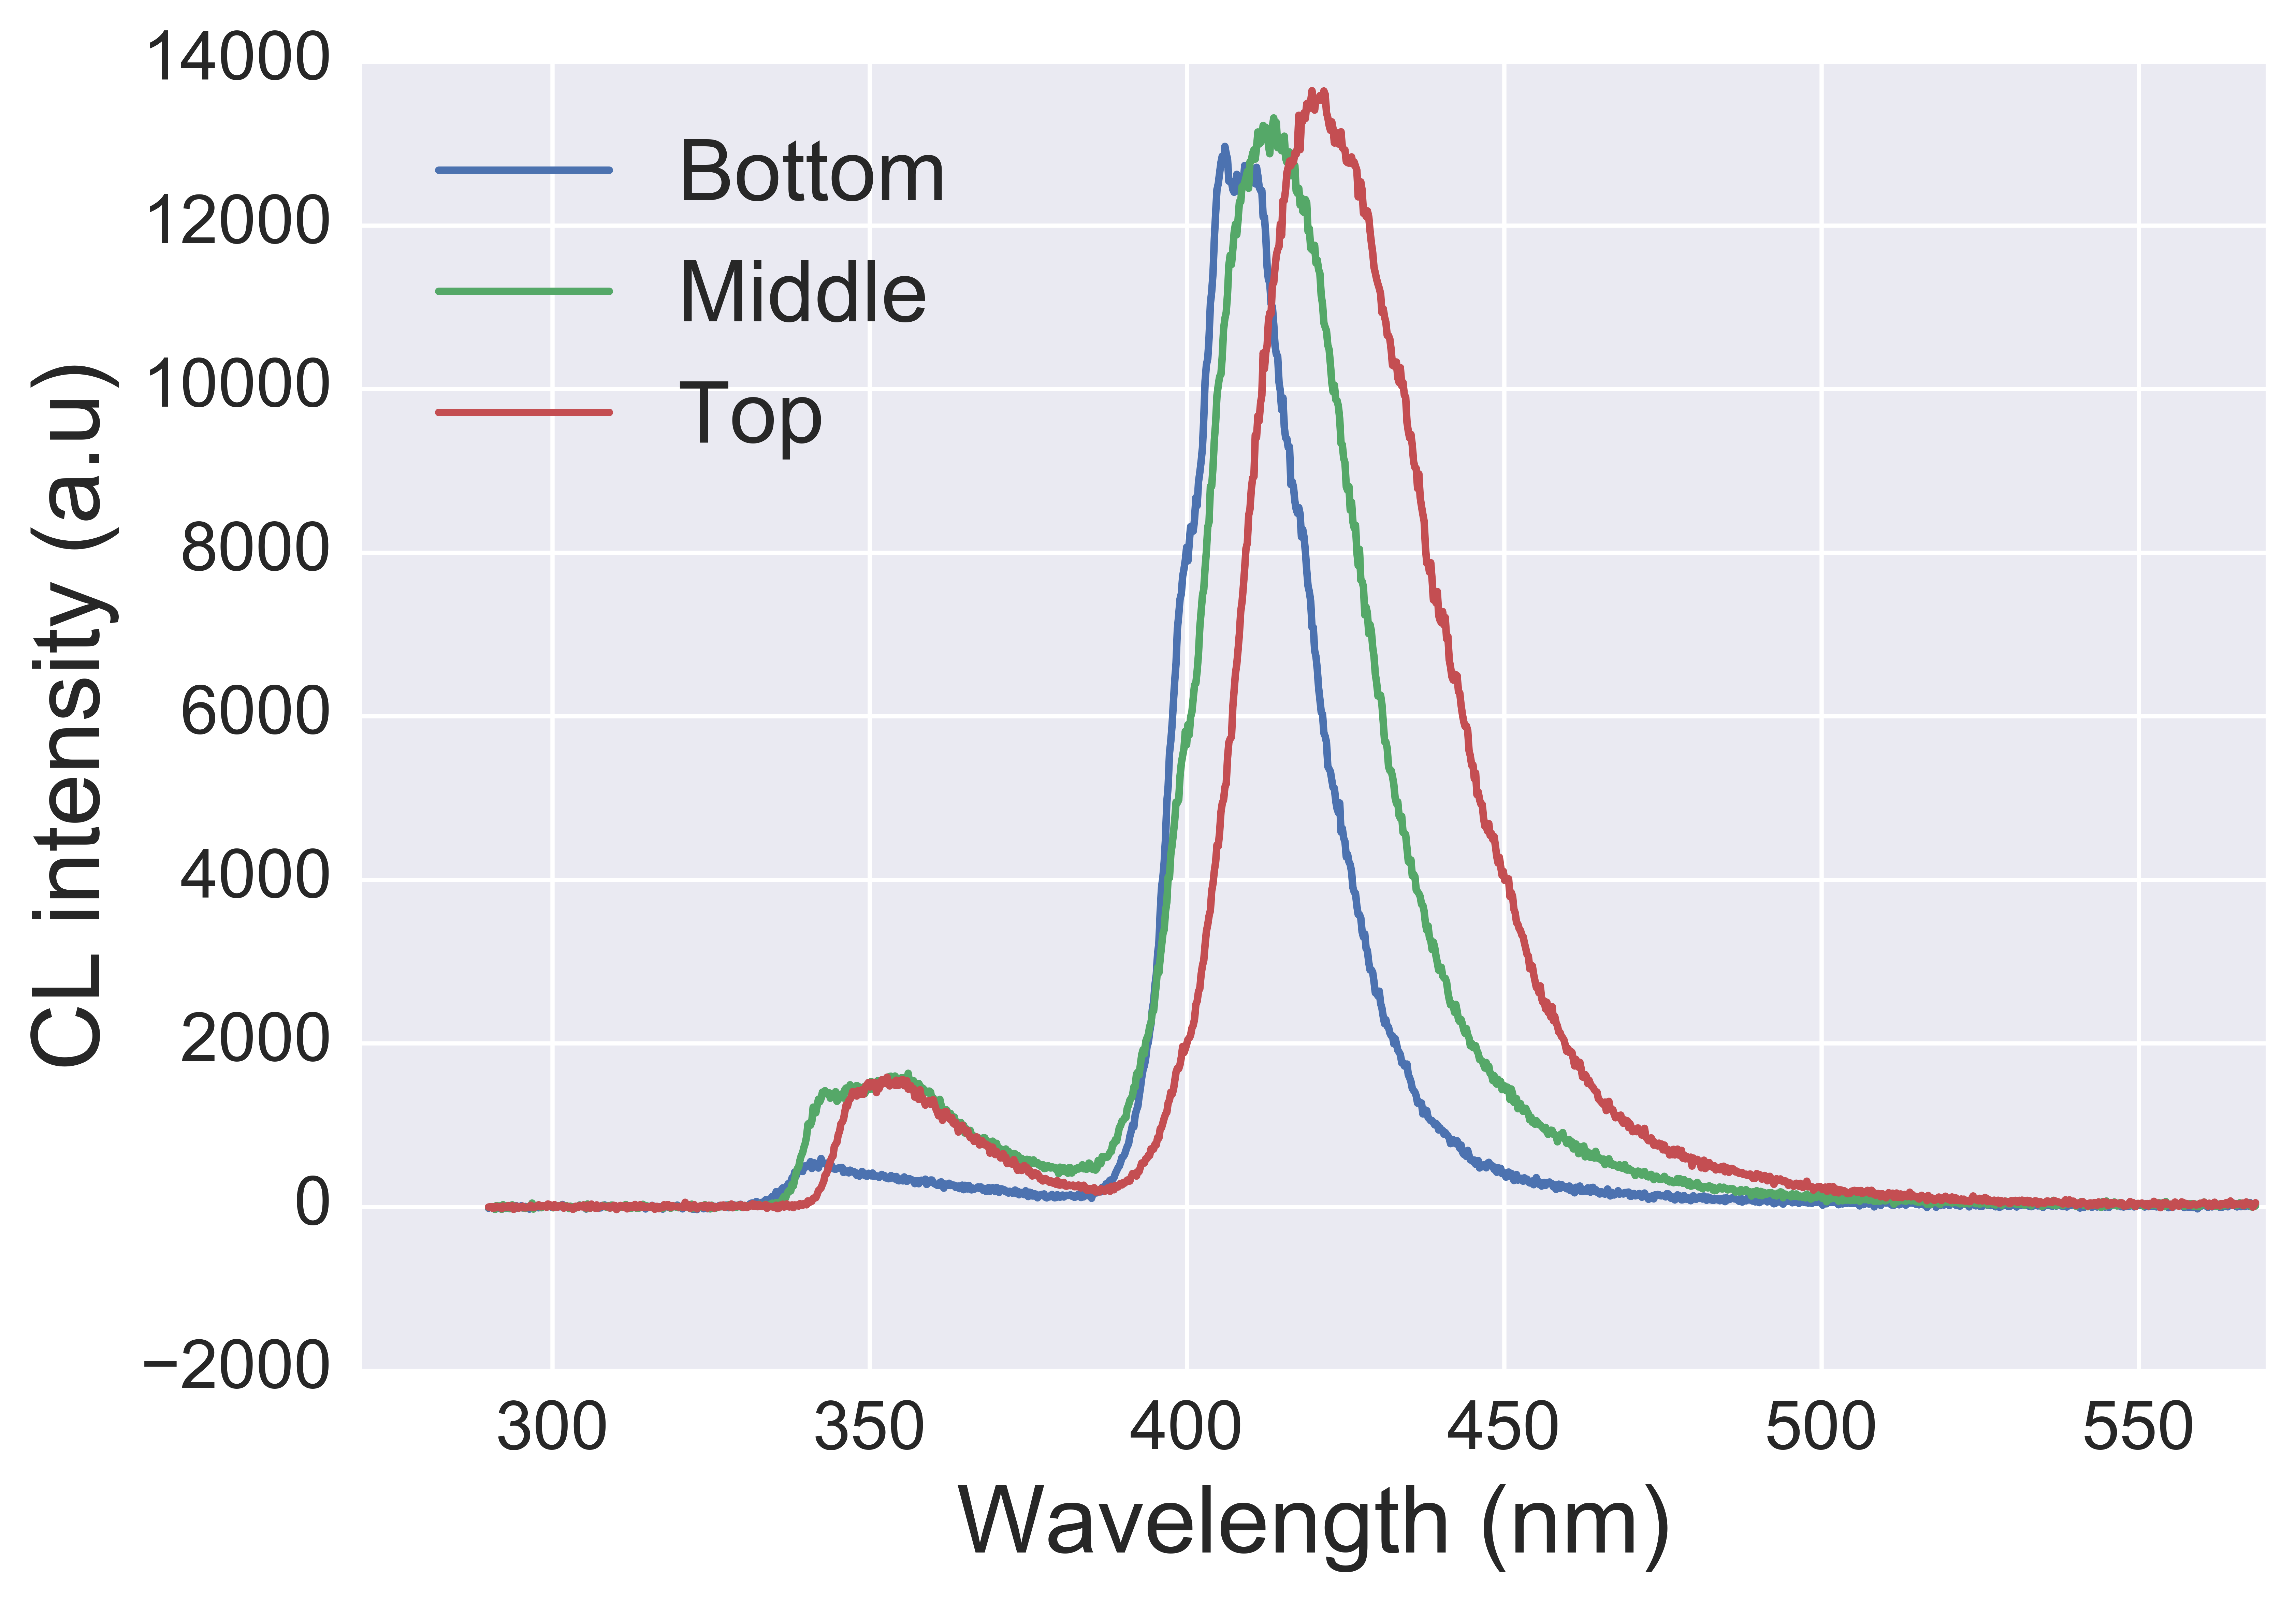
\includegraphics[width=1\linewidth]{Figs/Ch6/C6525}
		\caption{}
	\end{subfigure}%
	
	\caption{a) Panchromatic CL image showing the locations at which the CL spectra were taken b) CL spectra taken from the top, middle and bottom of the linescan with the respective normalisation factors shown in the legend.}
	\label{B-spectra}
\end{figure}
\FloatBarrier


\subsection{Microrod Structure and Composition}

\subsubsection{STEM}
\label{HAADF}
In order to elucidate the structural differences between the brightly emitting and dark portions of sample A we fabricated axial cross-sections of nanorod by FIB.

\begin{figure}[!h]
	\centering
	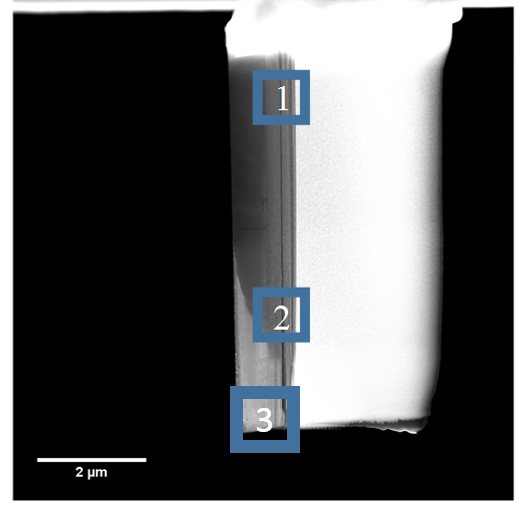
\includegraphics[width=0.5\textwidth]{Figs/Ch6/Aoverview}
	\caption{Low magnification STEM-HAADF image of a TEM lamella of the rod shown in Fig.\ref{sampleAscan} prepared by FIB.}
	\label{AHAADFoverview}
\end{figure}
\FloatBarrier 

A HAADF-STEM image of a sample prepared from a microrod harvested from sample A is shown in Figure \ref{AHAADFoverview}, with regions of interest denoted ‘1’ corresponding to a brightly emitting region and ‘2,3’ to dark region in the CL, as shown in Fig.\ref{sampleAscan}.b. 
STEM-HAADF images from region 1 are shown below in Fig.\ref{A12}, in which we can see the morphology of the non-polar QWs. These images show few structural perturbations in the rod morphology.

This is in stark contrast to Fig.\ref{A34}, which shows STEM-HAADF images taken in region 2. In this region we can see the QW stack and surface of the microrod are non-uniform, features which can be linked to the presence of the defect outlined in Fig.\ref{A34}.b which is likely to be a void defect as evidenced by the darker contrast in HAADF-STEM and the well defined void facets which are similar in morphology to those described by Yankovich \textit{et al.} \cite{Yankovich2012}.
\begin{figure}[!h]
	%\hspace*{-2cm}
	\begin{subfigure}[b]{0.45\textwidth}
		\centering
		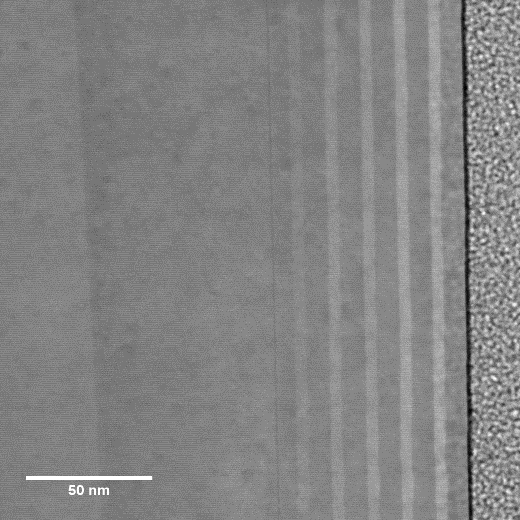
\includegraphics[width=1\linewidth]{Figs/Ch6/A1stem}
		\caption{}
		
	\end{subfigure}%
	\hspace*{1.2cm}
	\begin{subfigure}[b]{0.45\textwidth}
		\centering
		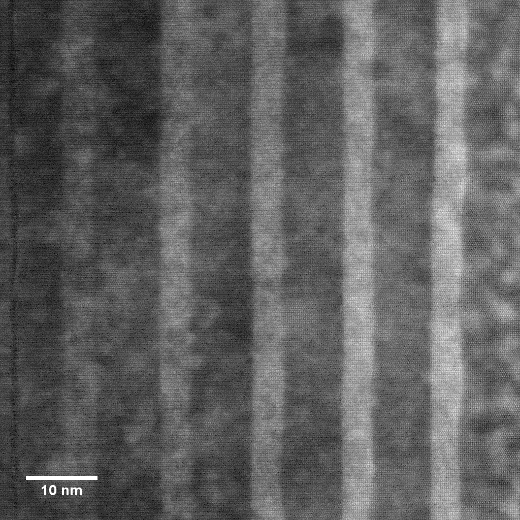
\includegraphics[width=1\linewidth]{Figs/Ch6/A2stem}
		\caption{}
	\end{subfigure}%
	
	\caption{STEM-HAADF images taken from region 1 of the rod from sample A.}
	\label{A12}
\end{figure}
\FloatBarrier

\begin{figure}[!h]
	%\hspace*{-2cm}
	\begin{subfigure}[b]{0.45\textwidth}
		\centering
		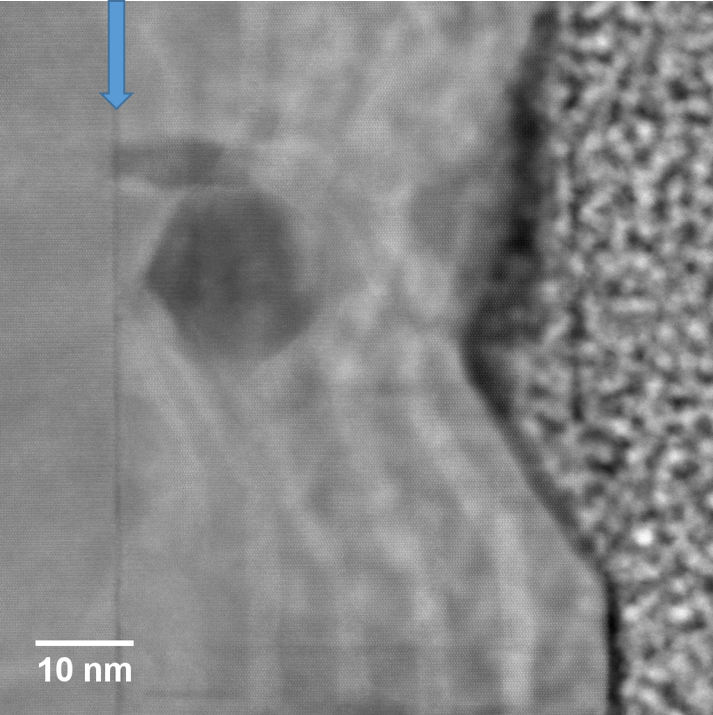
\includegraphics[width=1\linewidth]{Figs/Ch6/Astem4}
		\caption{}
		
	\end{subfigure}%
	\hspace*{1.2cm}
	\begin{subfigure}[b]{0.45\textwidth}
		\centering
		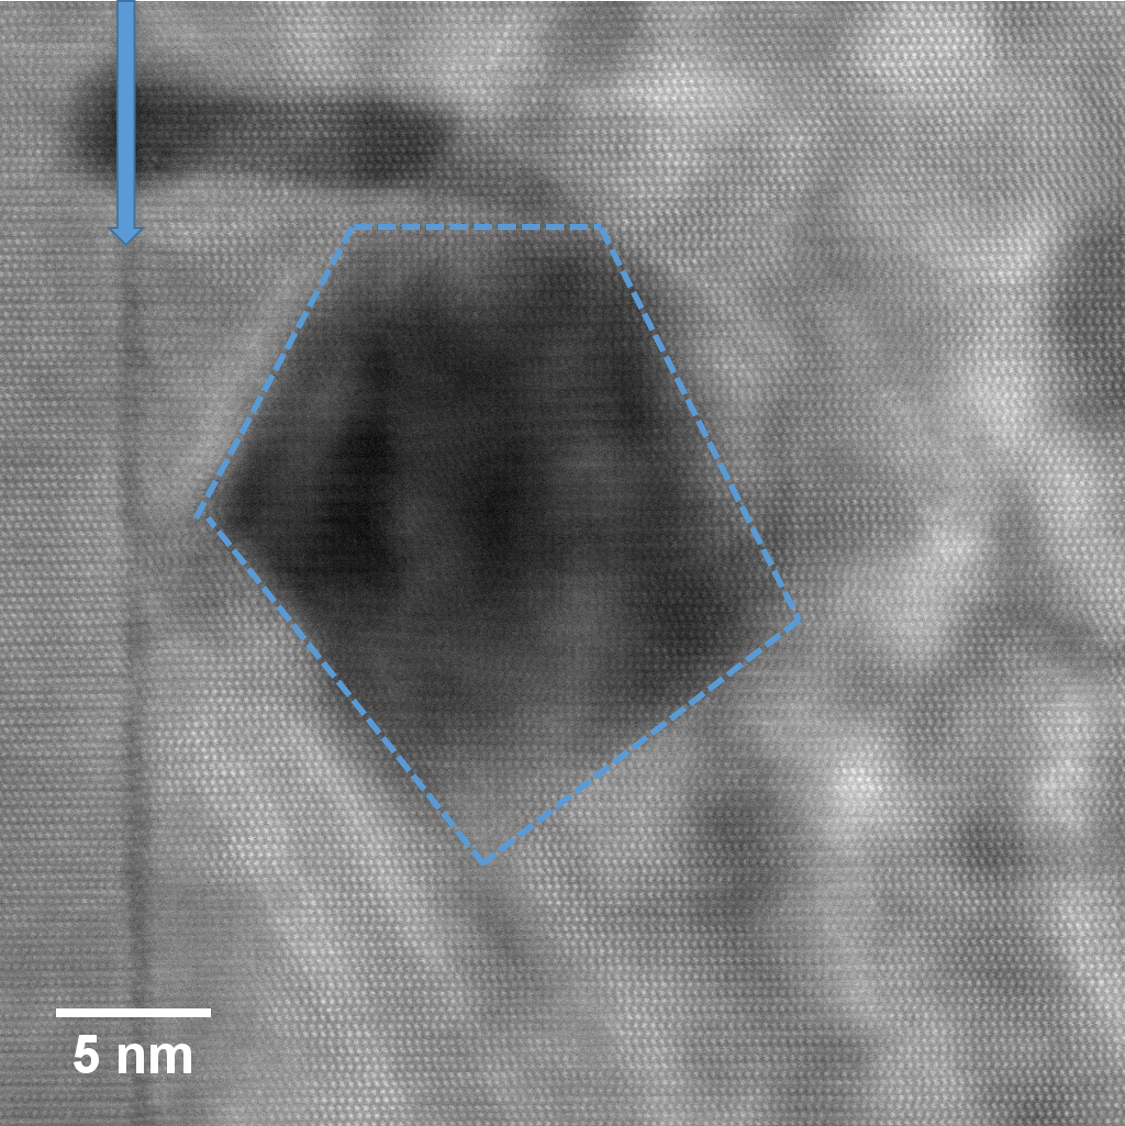
\includegraphics[width=1\linewidth]{Figs/Ch6/AvoidDF1}
		\caption{}
	\end{subfigure}%
	
	\caption{STEM-HAADF images taken from region 2 of the rod from sample A. The dark feature highlighted by the blue arrow is present in both the top and bottom regions of the rod. A large void defect is highlighted by the dashed lines.}
	\label{A34}
\end{figure}
\FloatBarrier

A STEM-BF image of region 2, highlighting the presence of voids (green arrows) and features providing darker contrast which are believed to be stacking faults (blue arrows) in this region, corresponding well to the lower region of rods from sample A which exhibited little to no emission in the CL. Although stacking faults themselves have been shown to emit luminescence (though only when examined at low temperature in the CL), they are often bound by partial dislocations which themselves act as non-radiative recombination centres \cite{Lahnemann2014}. The presence of voids is expected to increase the local density of surface states, thus also providing an increase in non-radiative recombination centres \cite{Yankovich2012}. Both types of defects are expected to quench CL emission, as seen at the bottom of microrods from sample A. 

\begin{figure}[!h]
	\centering
	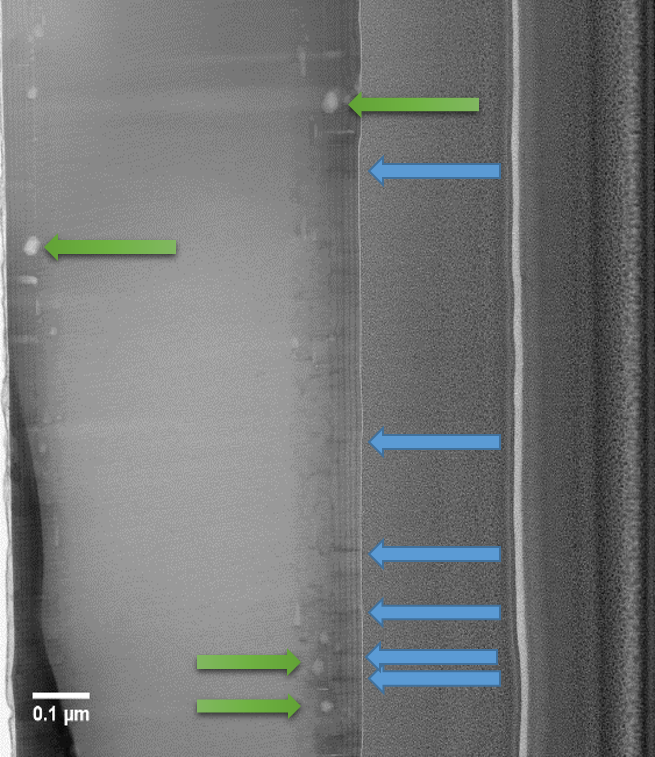
\includegraphics[width=0.8\textwidth]{Figs/Ch6/A3stem}
	\caption{ Low magnification STEM-BF image of region 2 from sample A, chosen to highlight the presence of stacking faults, which appear darker in contrast in STEM-BF.}
	\label{stembf}
\end{figure}

Fig.\ref{region3} shows a STEM-BF image taken of region 3 of the microrod. Here we can observe the microrod contains a high density of defects, and the microrod surface is highly corrugated due to the sub-optimal growth conditions. The approximate regions where the QW stack should be are delineated by the dashed lines. There is a distinct lack of the QW stack in these regions when compared to the image taken from region 2 shown in Fig.\ref{stembf}, indicating this region is also likely to show little to no CL emission, in good agreement with the CL data shown in Fig.\ref{sampleAscan}.b. Large voids are labelled using the red circles. 

\begin{figure}[!h]
	\centering
	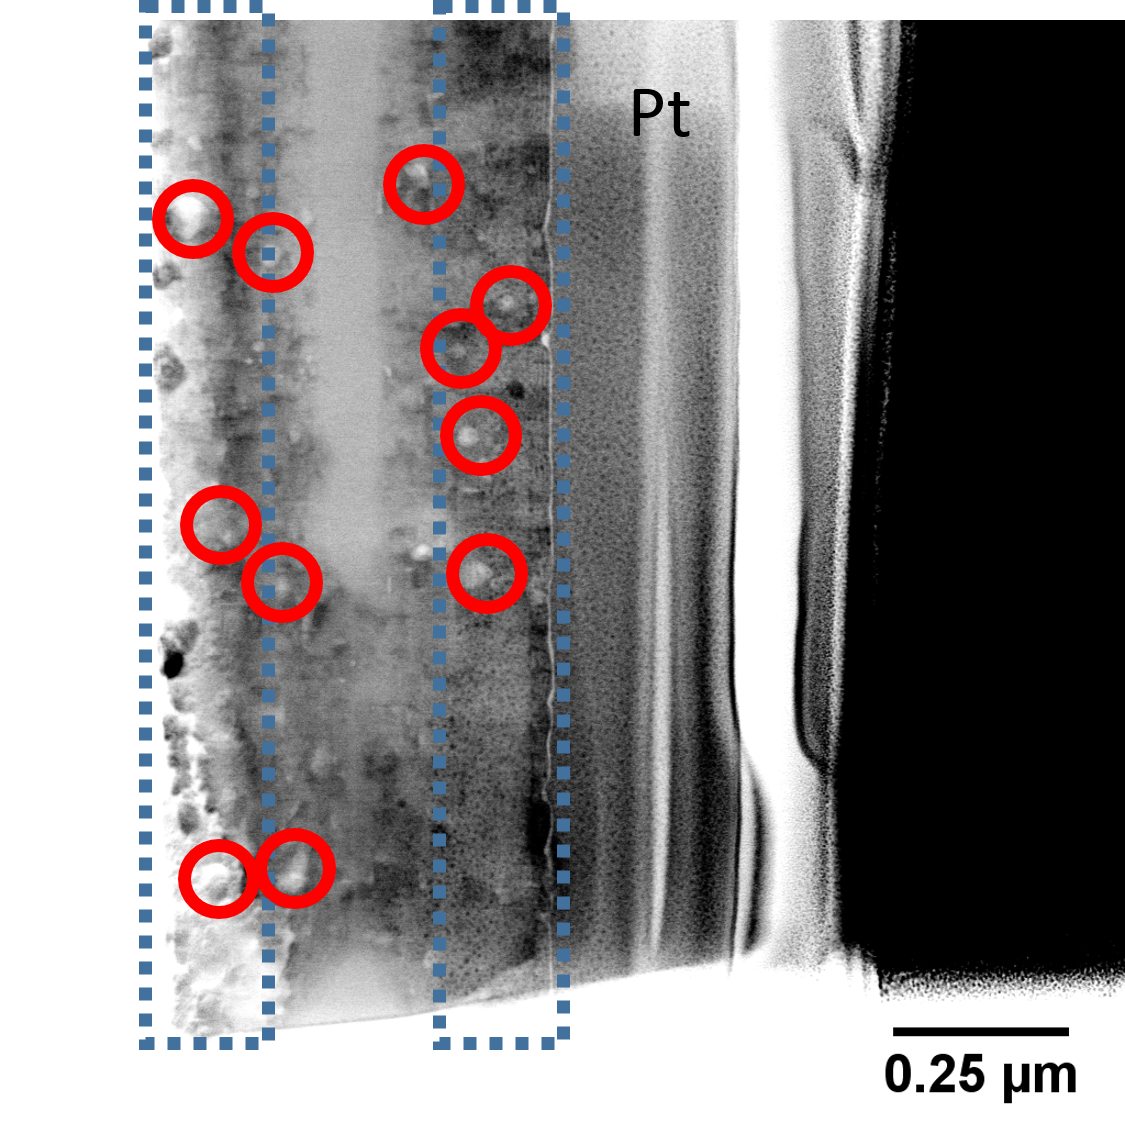
\includegraphics[width=0.8\textwidth]{Figs/Ch6/region3}
	\caption{ Low magnification STEM-BF image of region 3 from sample A, chosen to highlight the presence of voids and the non-uniform morphology of the microrod in this region. Large voids are labelled using the red circles, and the regions which are expected to contain the QW stack are delineated by the dashed lines.}
	\label{region3}
\end{figure}
\FloatBarrier

We repeated this analysis on a TEM lamella prepared from a rod harvested from sample B. STEM-HAADF images from the top and bottom of this rod are shown in Fig.\ref{Btopbot}.a. and b respectively. In these images once can observe that the bottom of this rod exhibits a morphology far more consistent with that at the top of the rod. Fig.\ref{Btopbot}.b shows a representative STEM-HAADF image of the bottom region of a microrod from sample B where the 'voids' seen at the bottom of the rod in Fig.\ref{A34} are present in far lower densities.
Some changes in morphology were still observed at the bottom of this rod, such as the bend in the QW stack shown in Fig.\ref{Btopbot}.b, delineated by the red ellipsoid. Fig.\ref{disturbance} shows further examples of non-uniformity in the QW stack in the bottom region of a microrod from sample B. In Fig.\ref{disturbance}.a we can see the distortion of the QW spacing in the stack Fig.\ref{disturbance}.b shows the disruption of the QW stack due to the presence of a void. These disruptions to the structure of the rod are however far fewer in number than those observed for the rod from sample A and shown in Fig.\ref{A34}. 

\begin{figure}[!h]
	%\hspace*{-2cm}
	\begin{subfigure}[b]{0.45\textwidth}
		\centering
		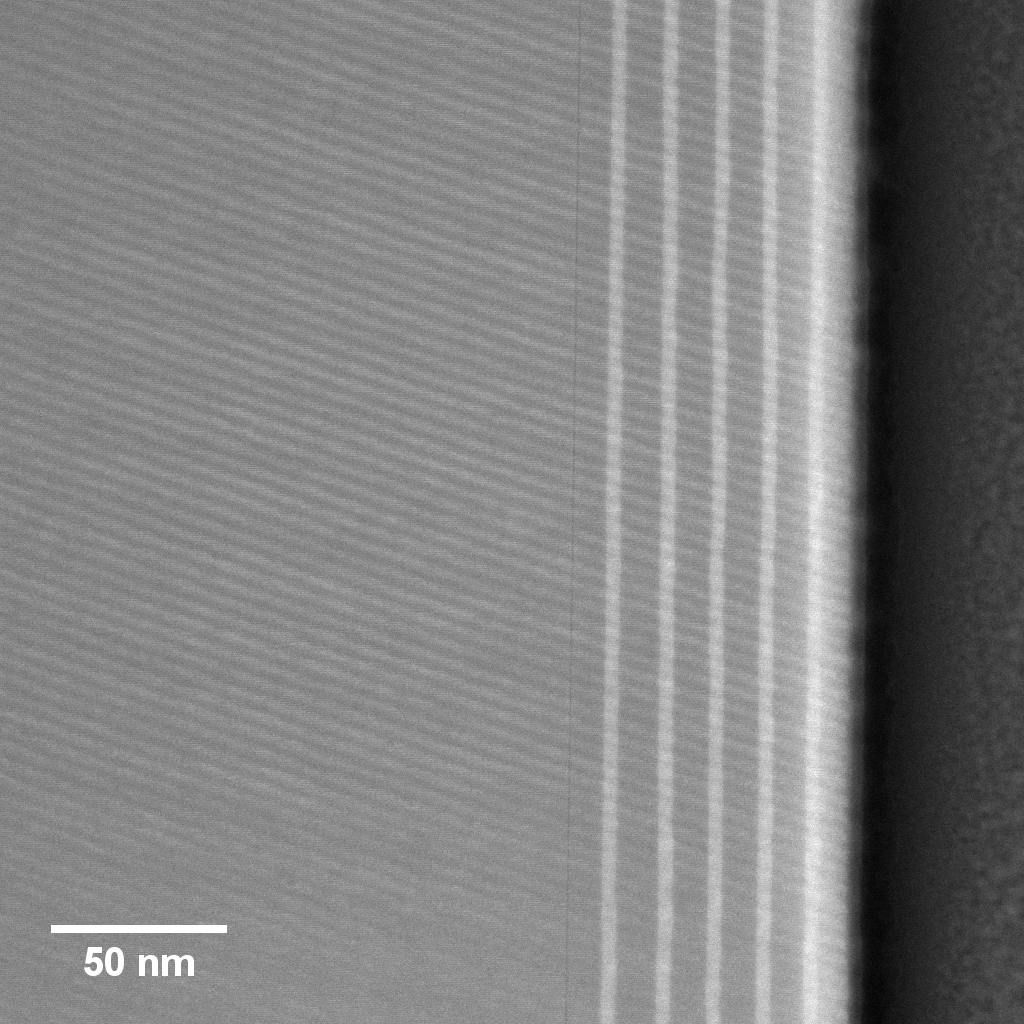
\includegraphics[width=1\linewidth]{Figs/Ch6/Bstem1}
		\caption{}
		
	\end{subfigure}%
	\hspace*{1.3cm}
	\begin{subfigure}[b]{0.45\textwidth}
		\centering
		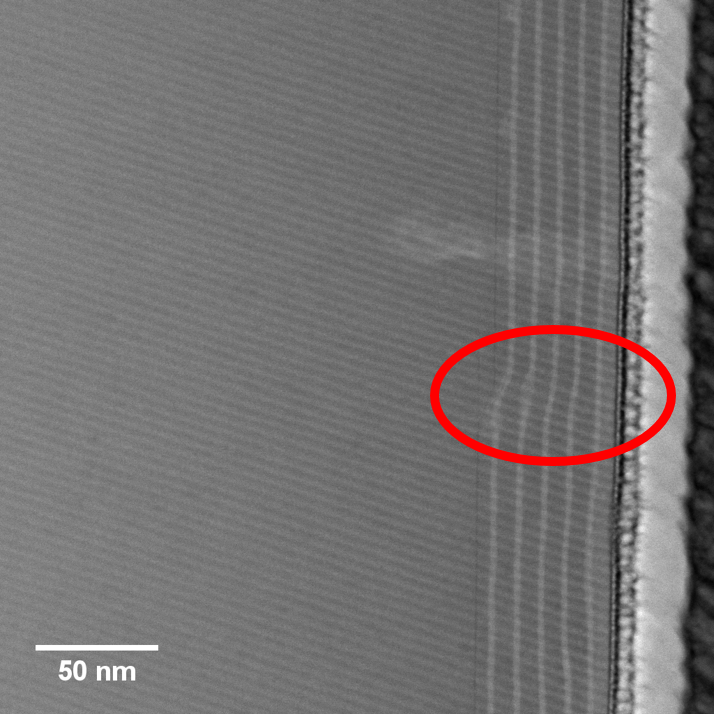
\includegraphics[width=1\linewidth]{Figs/Ch6/Bstembot}
		\caption{}
	\end{subfigure}%
	
	\caption{STEM-HAADF images taken from a) the top and b) the bottom of a rod harvested from sample B. }
	\label{Btopbot}
\end{figure}
\FloatBarrier

\begin{figure}[!h]
	%\hspace*{-2cm}
	\begin{subfigure}[b]{0.45\textwidth}
		\centering
		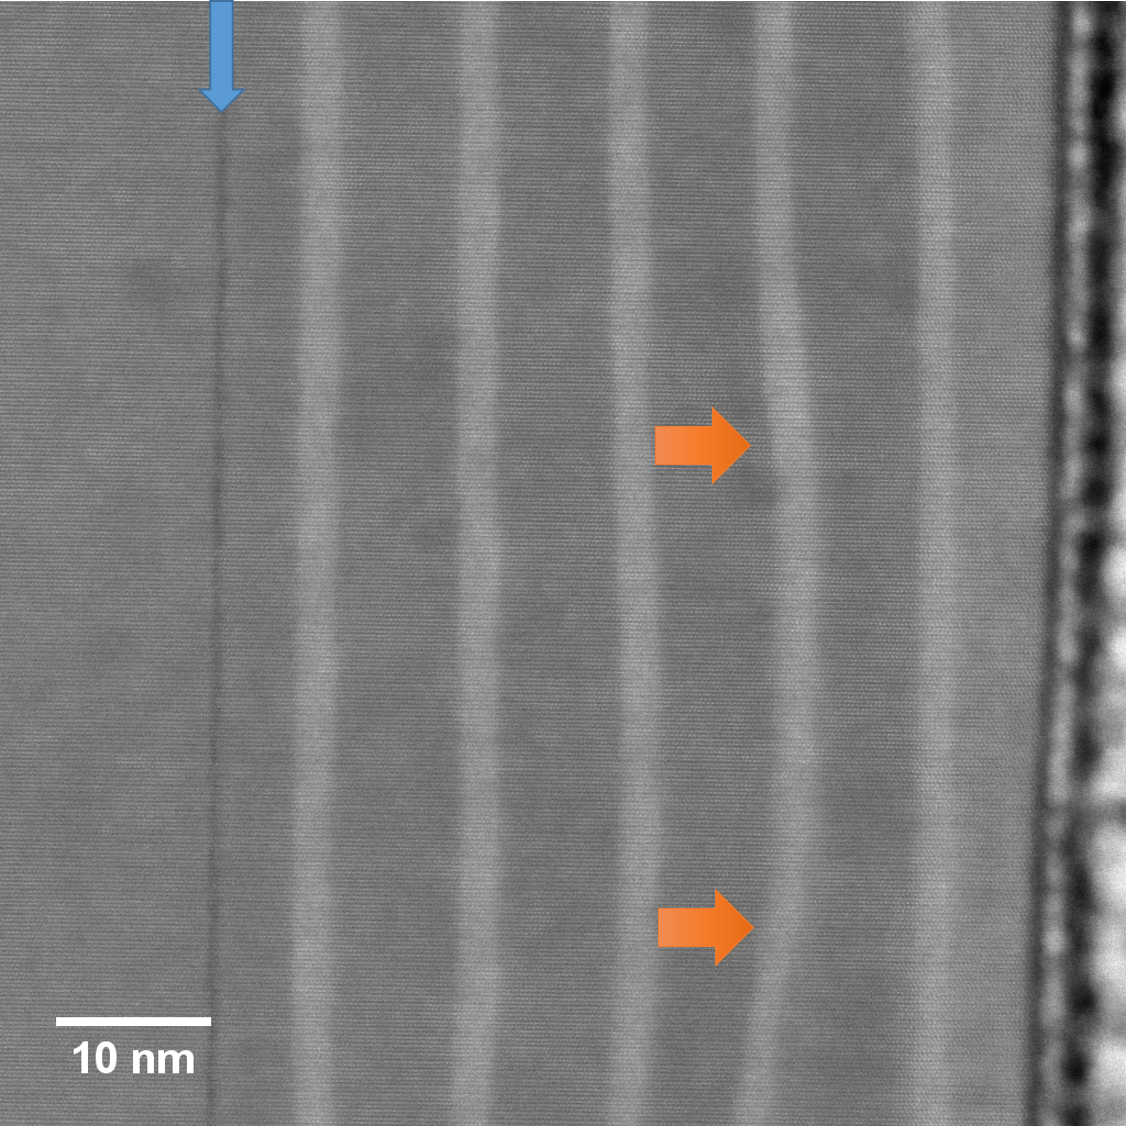
\includegraphics[width=1\linewidth]{Figs/Ch6/Bstem3}
		\caption{}
		
	\end{subfigure}%
	\hspace*{1.2cm}
	\begin{subfigure}[b]{0.45\textwidth}
		\centering
		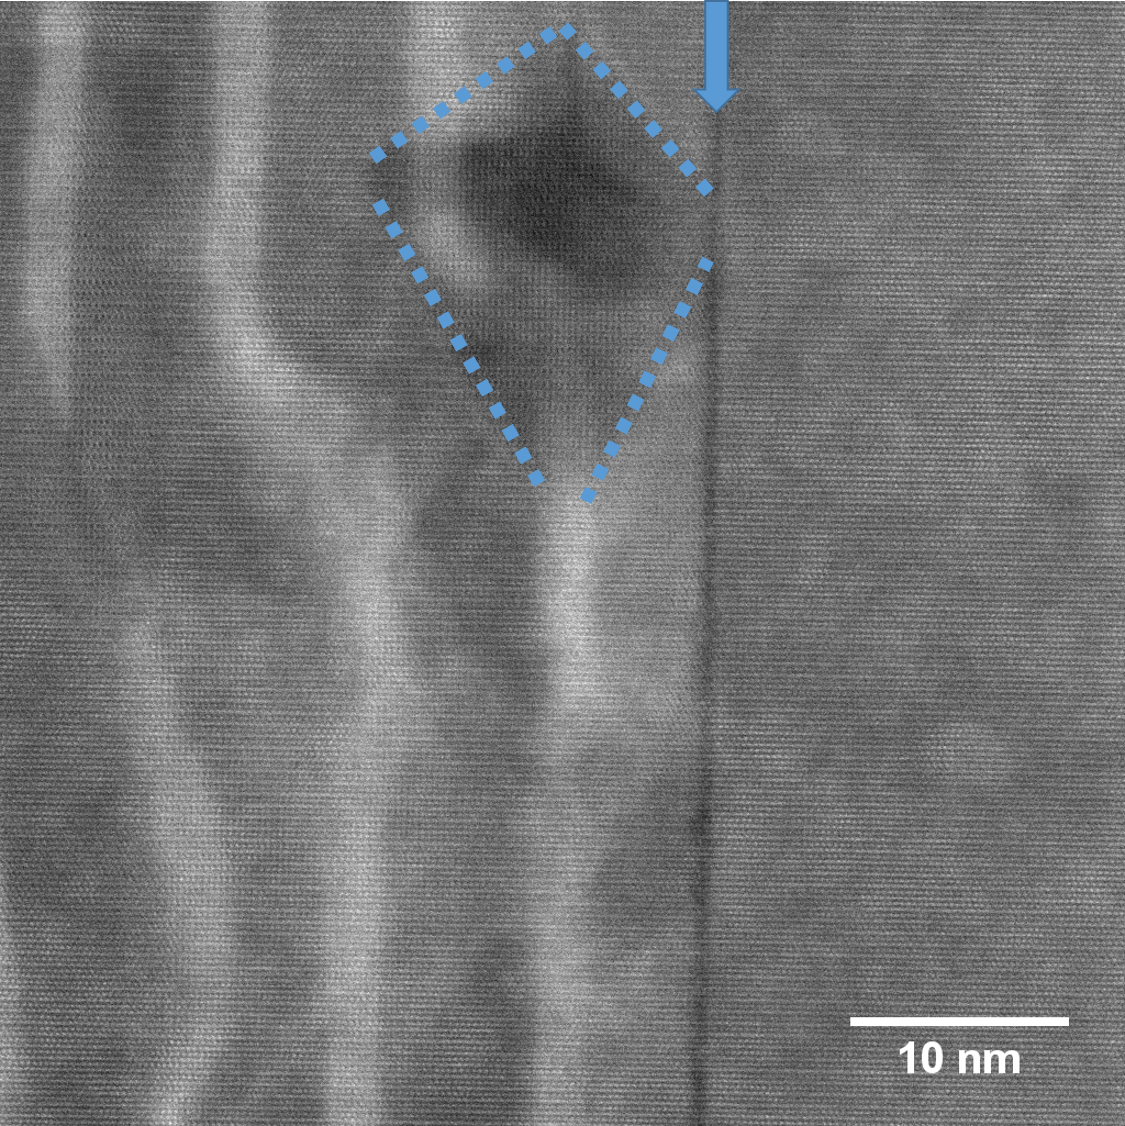
\includegraphics[width=1\linewidth]{Figs/Ch6/Bstem5}
		\caption{}
	\end{subfigure}%
	
	\caption{STEM-HAADF images of a) QW distortion and b) void related disruption of the QW stack in the lower region of a rod harvested from sample B.}
	\label{disturbance}
\end{figure}
\FloatBarrier

A common feature for rods taken from both samples is the dark contrast which can be observed preceding the first QW from the rod core and is highlighted using the blue arrows in figures \ref{A34} and \ref{disturbance}. The composition and origin of this feature will be investigated further in the rest of this work. 


\subsection{The Effect of Si on Microrod Growth}

Tessarek \textit{et al.} have reported the observation of a similar thin layer of dark contrast in STEM-HAADF images taken of microrods grown by MOVPE using a similar recipe to those described in section \ref{nanorod growth}. Using STEM-EDX, the authors reported the presence of Si in this layer and attributed this to the formation of a $\mathrm{SiN_{x}}$ layer present due to the supply of post-growth supply of ammonia \cite{Tessarek2014a}. In this section we will confirm the presence of Si in this layer in our microrods and examine the effect of this on microrod emission and morphology.


\subsubsection{Dual Plan-View TEM Lamella Preparation}

In order to characterise the $\mathrm{SiN_{x}}$ layer seen in the previous section, as well as to lay the ground work for future correlated experiments studying changes along the length of the microrods we devised a method of producing multiple TEM lamellae from a single rod using the FIB/SEM dual-beam, thus allowing for the characterisation of multiple sections along the growth axis. To our knowledge this is the first time this procedure has been carried out.
The methodology is presented in Fig.\ref{dual plan-view} which shows the following: the target rod is first welded onto the Omniprobe as is typical in FIB/SEM-based TEM lamella preparation methods. Following this, a stub consisting of Pt is deposited on the TEM grid, in order to ensure the final axial section is not obscured by the grid itself when examined in the TEM due to the small cross-sectional dimensions of the rod as shown in Fig.\ref{dual plan-view}.a. The rod is then attached onto the stub at the location along the rod from which we wish to produce a sample (shown in Fig.\ref{dual plan-view}.b). This rest of the rod is then released using ion-beam milling as shown in Fig.\ref{dual plan-view}.c, thus allowing for this process to be repeated as many times as the length of the rod will allow. This section of the rod is then thinned down to electron transparency using standard FIB sample preparation methods. A prepared sample is shown in Fig.\ref{dual plan-view}.d. We estimate that this method allows for sections to be cut at intervals of 400-500 nm along microrod. In this particular case we have performed the process twice, producing one axial sample from the top and one from the bottom of rods from both sample A and B.

\begin{figure}[h]
	\begin{subfigure}[b]{0.48\textwidth}
		\centering
		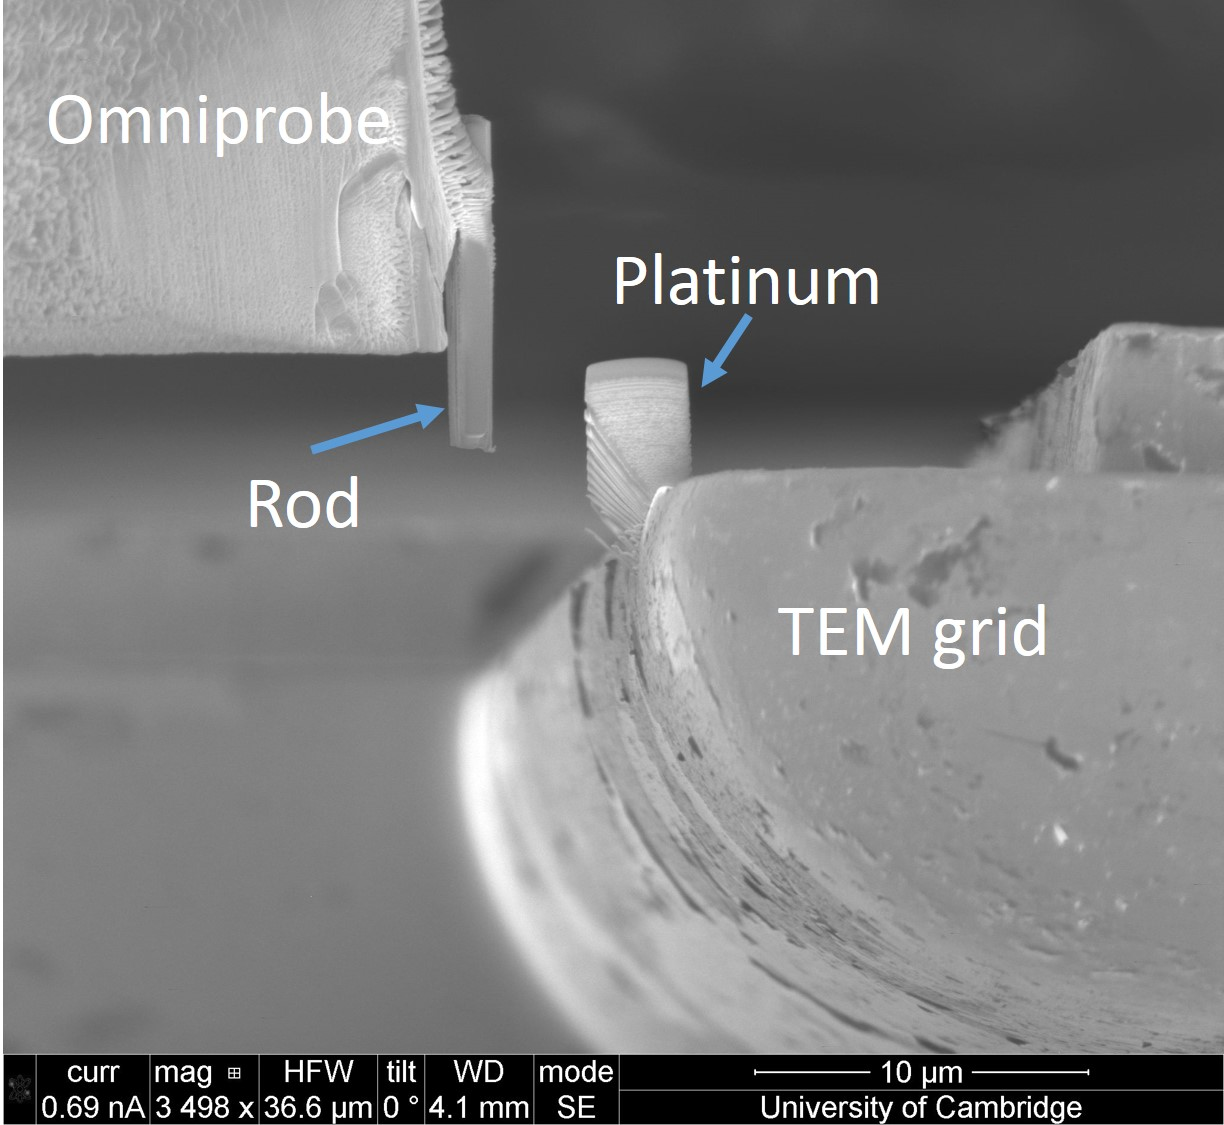
\includegraphics[width=1\linewidth]{Figs/Ch6/region1_016}
		\caption{Approach}
	\end{subfigure}%
	\hspace*\fill
	\begin{subfigure}[b]{0.48\textwidth}
		\centering
		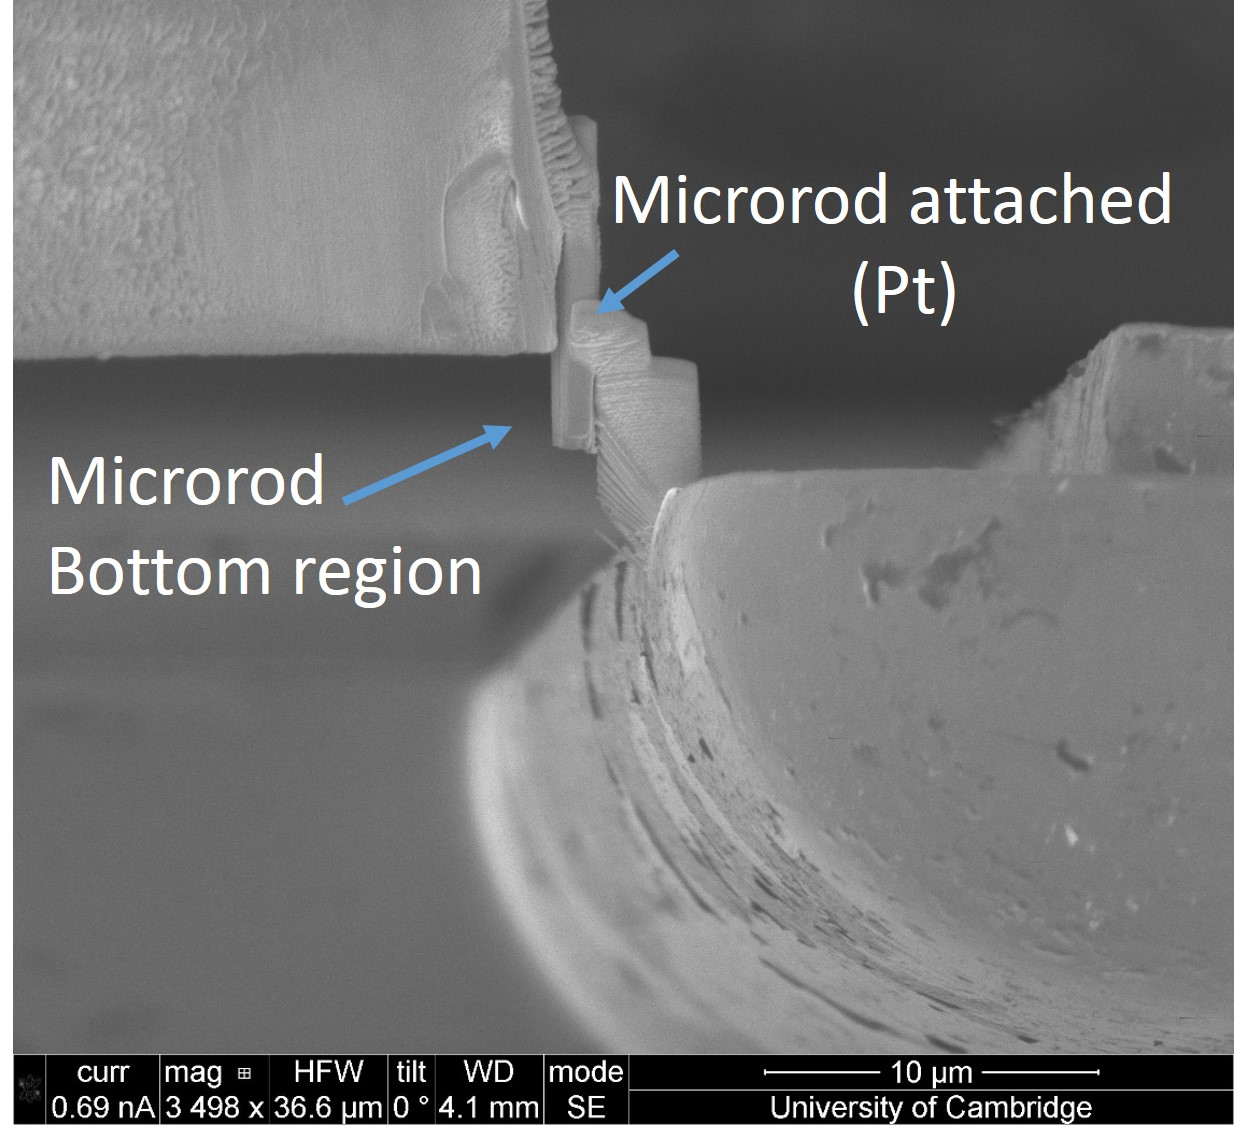
\includegraphics[width=1\linewidth]{Figs/Ch6/region1_017}
		\caption{Welding}		
	\end{subfigure}%
	
	\medskip
	\begin{subfigure}[b]{0.48\textwidth}
		\centering
		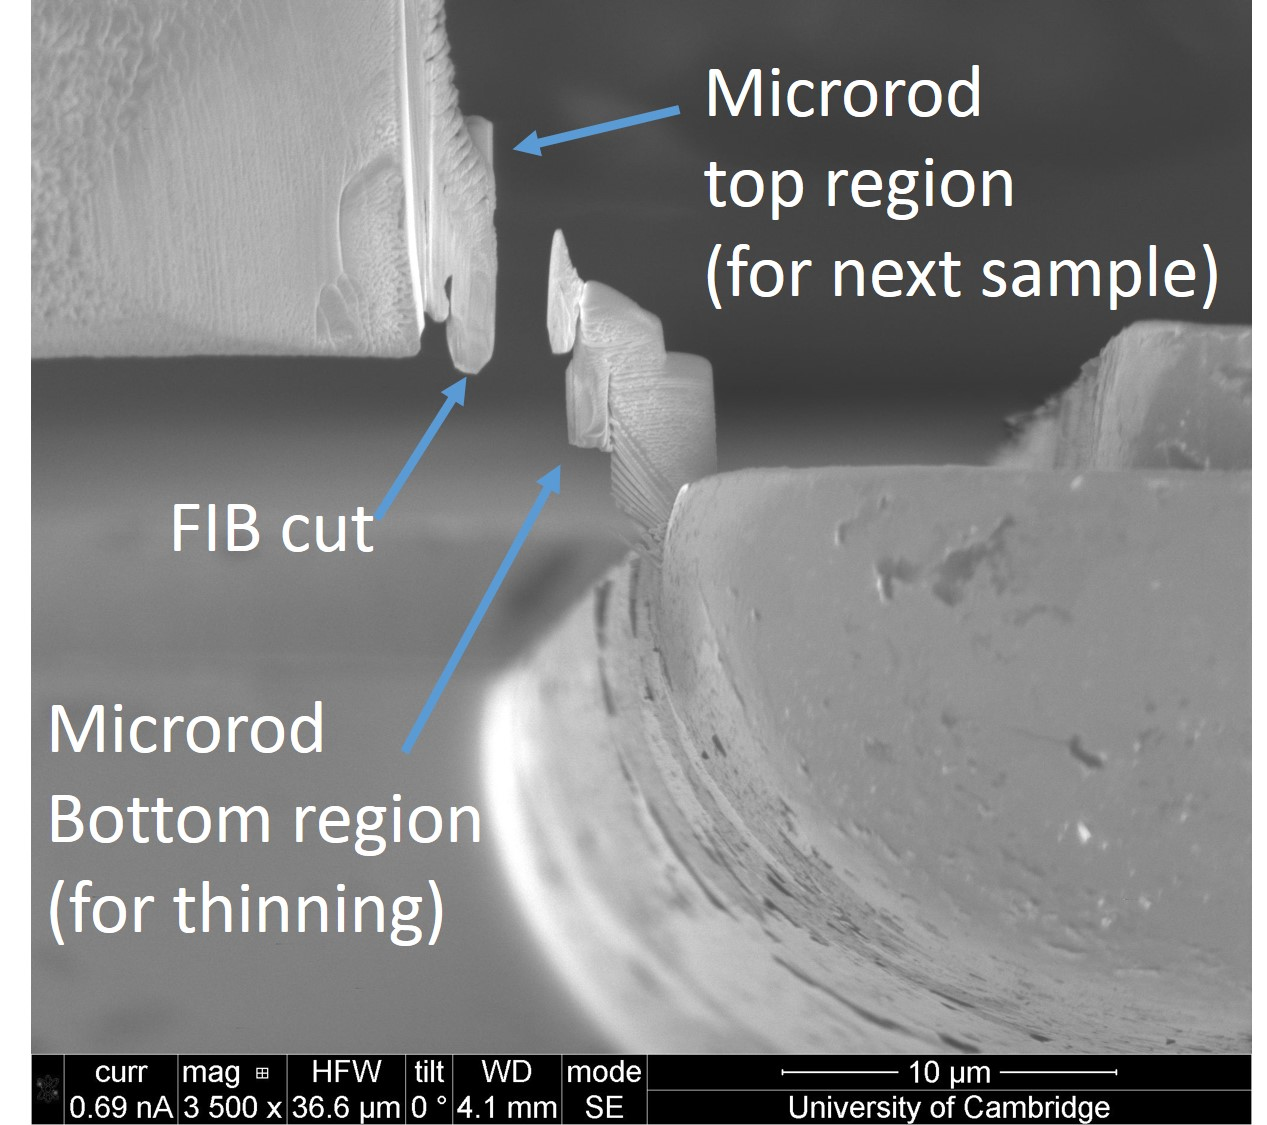
\includegraphics[width=1\linewidth]{Figs/Ch6/region1_018}
		\caption{Release}
	\end{subfigure}%
	\hspace*\fill
	\begin{subfigure}[b]{0.48\textwidth}
		\centering
		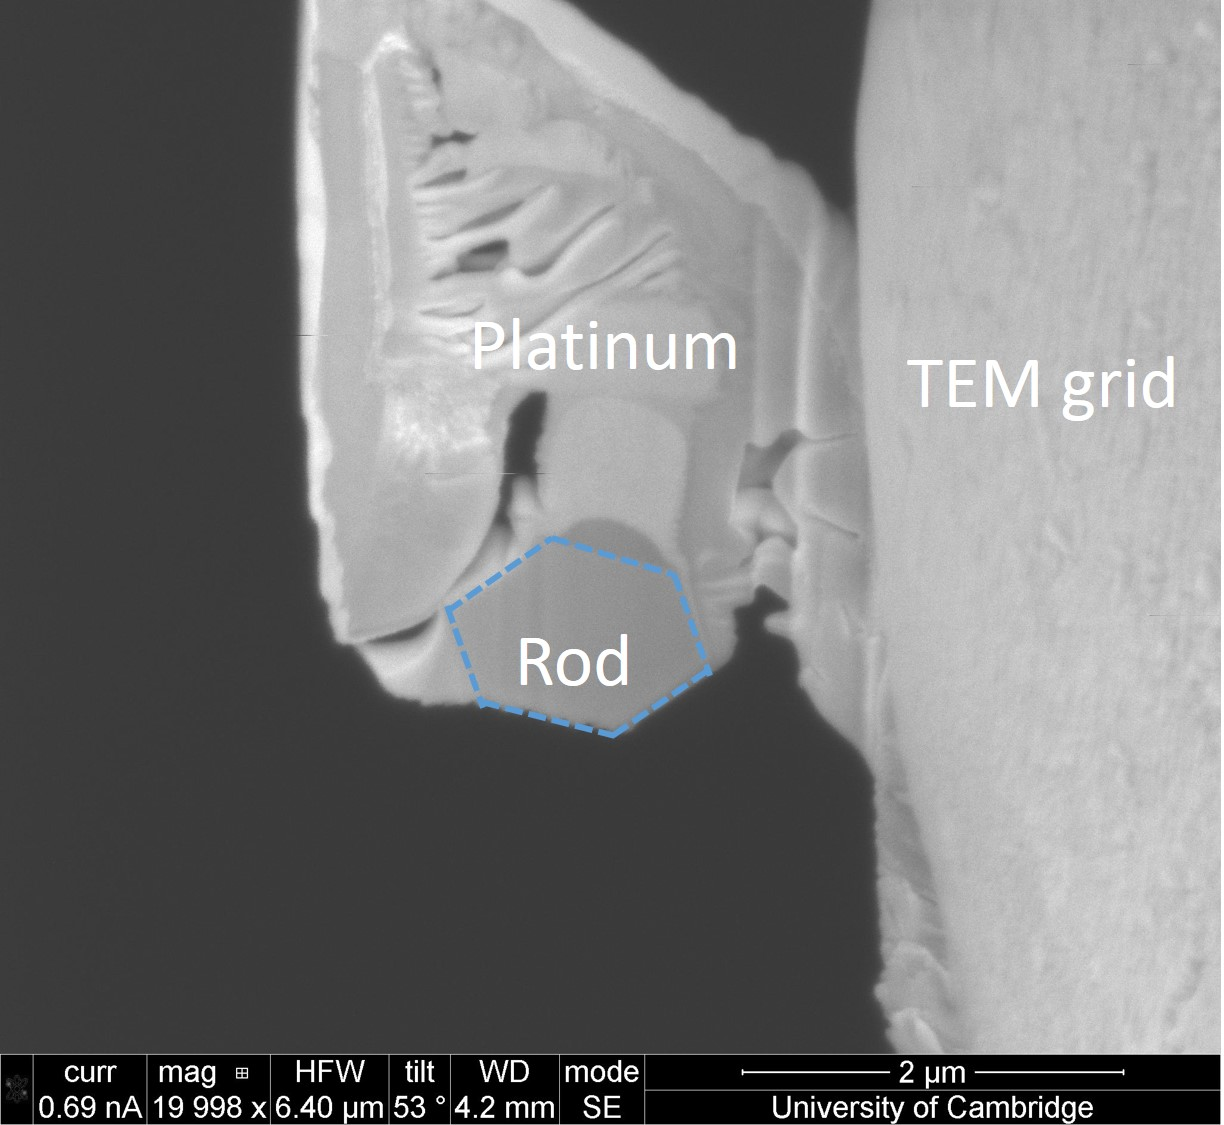
\includegraphics[width=1\linewidth]{Figs/Ch6/region1_023}
		\caption{Final lamella}		
	\end{subfigure}%
	\caption{Axial cross-section lamella preparation. The three steps shown above (a, b and c) may be repeated as many times as the length of the rod allows, allowing for the preparation of multiple cross-sections from the same rod. d) shows a finished sample, viewed along the microrod growth axis (this image is taken at 45 degrees relative to the other three images in this set).}
	\label{dual plan-view}
\end{figure}
\FloatBarrier

\subsubsection{Si Content Quantification}
As discussed in section \ref{nanorod growth}, the two microrod samples were grown with different silane flows. In section \ref{HAADF} we have examined structural differences between the top and bottom of both rods, corresponding to differences to CL emission homogeneity as shown in \ref{rod emission}. Furthermore we have shown the presence of a feature preceding the QW stack in STEM-HAADF which is believed to be a $\mathrm{SiN_{x}}$ layer resulting from the silane flow necessary to enhance vertical rod growth \cite{Tessarek2014a}. In this section we will use STEM-EDX in order to confirm the presence of Si in this layer, and investigate the relationship between the Si content and structural and emissive properties of the rods. For this experiment we have prepared plan-view samples from the top and bottom of rods harvested from both sample A and B.
Fig.\ref{AbotEDX}.a shows a portion of a plan-view TEM sample prepared from the bottom of a rod from sample A. The radial growth of the rod beyond the dark layer (labelled using the blue arrows) seems to have been hindered, heavily disrupting the growth of QWs and resulting in a smaller rod radius, in this case the distance between the thin, dark layer and the edge of the rod is approximately 20 nm.

\begin{figure}[h]
	\centering
	\includegraphics[width=0.6\textwidth]{Figs/Ch6/abotdf}
	\caption{a) STEM-HAADF image of a TEM sample prepared from the bottom of a rod from sample A. The contrast in this image has been enhanced for clarity.}
	\label{AbotDF}
\end{figure}
\FloatBarrier

 
Fig.\ref{AbotEDX}.b shows the presence of a low In content (2.0-3.5 \%) in this region, suggesting the growth conditions at the bottom of rods from sample A can result in the formation of a thick low In content layer rather than a QW stack. This disruption in the growth of the QW stack has been shown in Fig.\ref{region3}. As such the low CL emission observed at the bottom of rods harvested from sample A may be due not only to the presence of voids and defects disrupting the QW stack morphology and acting as non-radiative recombination centres, but simply also a lack of QW formation. Fig.\ref{AbotEDX}.c shows the Si content extracted from the EDX map, thus confirming the presence of Si in the layer generating dark contrast in the STEM-HAADF images. The Si content detected in this layer in this region is in the range 7-10\%.

\begin{figure}[h]
	\centering
	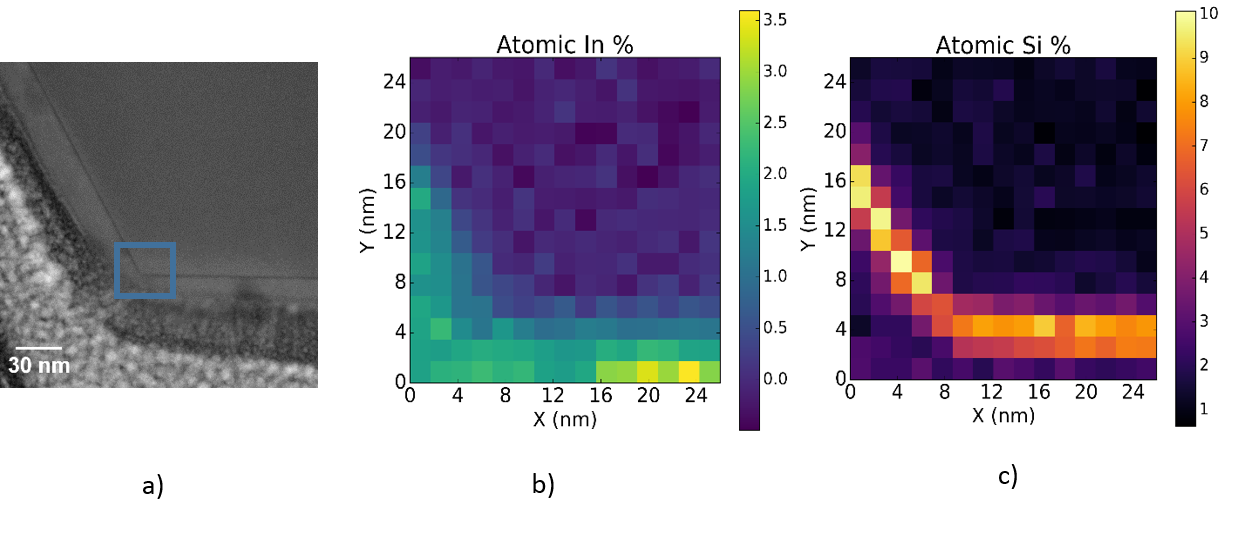
\includegraphics[width=1\textwidth]{Figs/Ch6/A-bot-EDX}
	\caption{a) STEM-HAADF image of a TEM sample prepared from the bottom of a rod from sample A b) In and c) Si content extracted from EDX maps taken from the region labelled by the blue box.}
	\label{AbotEDX}
\end{figure}
\FloatBarrier

In the interpretation of these results it is important to consider the possibility this layer may be an extremely highly Si-doped GaN layer rather than a $\mathrm{SiN_{x}}$ layer. However, the results shown in Fig.\ref{AbotEDX}.b would indicate an Si doping concentration of approximately $4.5 \times 10^{21} cm^{3}$, an order of magnitude higher than the highest reported Si doping concentration of $2.8 \times 10^{20} cm^{3}$ in MBE grown nanowires \cite{Fang2015} which was already reported to exceed the theoretically predicted Si solubility limit \cite{Neugebauer2003}. Furthermore, the N-rich conditions (see section \ref{nanorod growth}) for the growth of these microrods is likely to result in the formation of a $\mathrm{SiN_{x}}$ \cite{Neugebauer2003}. As such, we attribute this dark layer seen in the STEM-HAADF images to the presence of a $\mathrm{SiN_{x}}$ layer. In light of this, it is also important to consider the quantified Si content of this layer is likely to be an underestimate: due to the fundamental limitation of electron-probe size in the microscope neighbouring layers are likely to be sampled with the $\mathrm{SiN_{x}}$ layer, resulting in an underestimate of the Si content in the layer. Markut \textit{et al.} report the stochiometry of the $\mathrm{SiN_{x}}$ mask as a $\mathrm{SiGaN_{3}}$ monolayer \cite{Markurt2013}, on this basis of which we expect the upper bound on the detected Si content to be 20 \%, though it is important to note that the analysis performed by Markut \textit{et al}. was performed on a \textit{c}-plane structure and may differ slightly from that present on the \textit{m}-plane facets of the microrods studied here. However, the porous morphology of the $\mathrm{SiN_{x}}$ mask \cite{Kappers2007} is crucial in interpreting the Si content detected by EDX here: as a result of this morphology we can expect the Si content to effectively be a measure of $\mathrm{SiN_{x}}$ coverage along the depth of the TEM lamella, thus providing us with a manner in which to quantitatively compare $\mathrm{SiN_{x}}$ coverage at different regions of the microrod.
Fig.\ref{AtopEDX}.a. shows a STEM-HAADF image of a plan-view TEM sample prepared from the top of the same rod shown in Fig.\ref{AbotEDX}.a. Here we can see the QW stack has been formed, and the radius of the rod is larger beyond the $\mathrm{SiN_{x}}$ layer. Fig.\ref{AtopEDX} shows the Si content of the $\mathrm{SiN_{x}}$ layer extracted from the EDX map, which in this region of the rod lies in the 2-5 \% range, far lower than that detected in Fig.\ref{AbotEDX}.b at the bottom of the rod. We can thus hypothesize that the coverage of the $\mathrm{SiN_{x}}$ layer has an effect on the morphology of the QW stack and thus the optical properties of the rod.

\begin{figure}[!h]
	\centering
	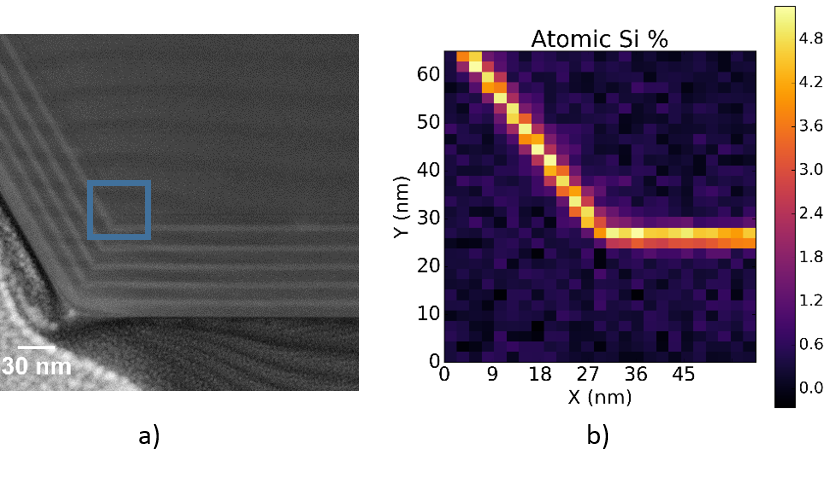
\includegraphics[width=1\textwidth]{Figs/Ch6/A-top-EDX}
	\caption{a) STEM-HAADF image of a TEM sample prepared from the top of a rod from sample A b) Si content extracted from EDX maps take from the region labelled by the blue box.}
	\label{AtopEDX}
\end{figure}
\FloatBarrier 

The effects of $\mathrm{SiN_{x}}$ coverage on the structural and optical properties of the rods are supported by the figures \ref{BbotEDX} and \ref{BtopEDX} which show the same experiment performed on top and bottom regions of a microrod from sample B. As noted previously, rods from sample B exhibited CL emission over the majority of the length of the rod as opposed to only the upper portion for rods from sample A. Fig.\ref{BbotEDX}.b shows the Si content of the $\mathrm{SiN_{x}}$ layer in the bottom portion of a rod harvested from sample B, which lies in the range 3-6.4\% in the region examined. This Si content is very similar to that shown in Fig.\ref{BtopEDX}.b, which shows the value extracted in the upper region of the same rod which lies in 2.4-5.6\%. As expected, this 'low' Si content corresponds to regions with good QW morphology and CL emission which are present along the majority of the rod length for sample B.

\begin{figure}[!h]
	\centering
	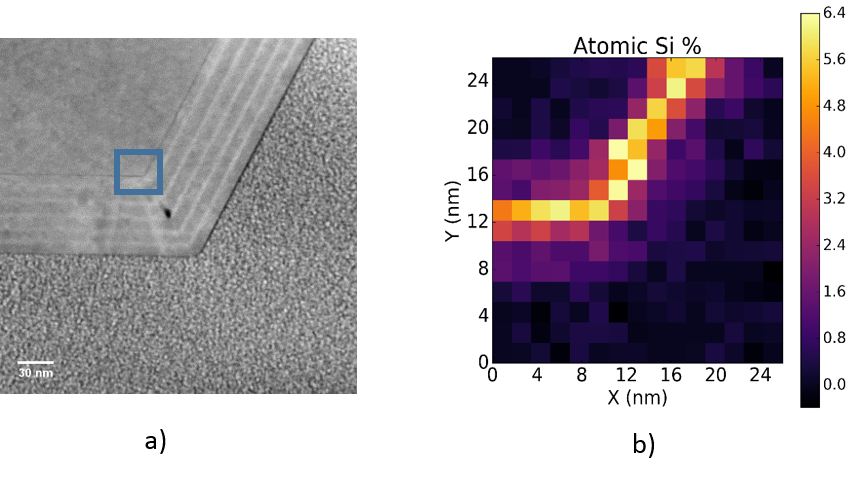
\includegraphics[width=0.87\textwidth]{Figs/Ch6/B-bot-EDX}
	\caption{a) STEM-HAADF image of a TEM sample prepared from the bottom of a rod from sample B b) Si content extracted from EDX maps take from the region labelled by the blue box.}
	\label{BbotEDX}
\end{figure}
\FloatBarrier 
\begin{figure}[!h]
	\centering
	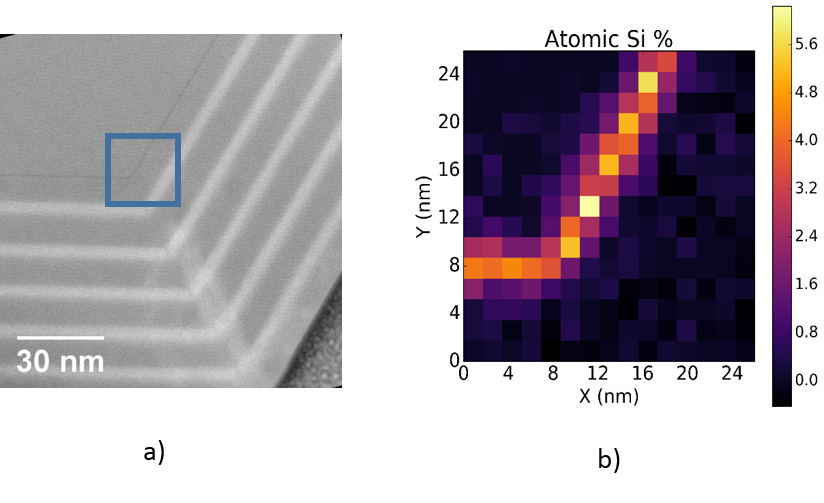
\includegraphics[width=0.87\textwidth]{Figs/Ch6/B-top-EDX}
	\caption{a) STEM-HAADF image of a TEM sample prepared from the top of a rod from sample B b) Si content extracted from EDX maps take from the region labelled by the blue box.}
	\label{BtopEDX}
\end{figure}
\FloatBarrier 

The results from the plan-view samples are summarised in the table below.

\begin{minipage}{\linewidth}
	\centering
	\captionof{table}{$\mathrm{SiN_{x}}$ layer Si atomic \%} \label{tab:title} 
	\begin{tabular}{c c c c} 
		\hline 
		 & Bottom & Top [0.5ex] \\
		\hline\hline 
		Sample A & 7-10 \% & 2-5 \%  \\
		\hline
		Sample B & 3-6.4 \% & 2.4-5.6 \% \\
		\hline
	\end{tabular}
	\bigskip
\end{minipage}

\subsubsection{Discussion}
\label{discussSiN}
The use of silane to generate an $\mathrm{SiN_{x}}$ nanomask during epitaxial GaN growth was first reported by Venn\'egu\`es \textit{et al.} \cite{Vennegues1998}. Since then, the use of an $\mathrm{SiN_{x}}$ as an interlayer for the reduction of threading dislocation densities in III-nitride epitaxial films has been thoroughly investigated \cite{Bottcher2003,Kappers2007,Johnston2009}. Tanaka \textit{et al.} also demonstrated the use of silane as a surfactant in inducing three-dimensional growth resulting in GaN quantum dots (QDs) with dimensions of approximately 100 nm on an AlGaN surface \cite{Tanaka1996}. Oliver \textit{et al.} have also exploited this effect in inducing the growth of InGaN islands on GaN, noting an increase in InGaN island density with increasing pre-growth silane exposure time \cite{OliverVanderLaakKappersEtAl2008}. The porous $\mathrm{SiN_{x}}$ layer resulting from the introduction of silane results in islands grown from the holes in the mask whilst the mask itself hinders the growth of the epitaxial layer, thus inducing 3D growth. This is shown in Fig.\ref{3Dgrowth}.

\begin{figure}[th]
	%\hspace*{-2cm}
	\begin{subfigure}[b]{0.48\textwidth}
		\centering
		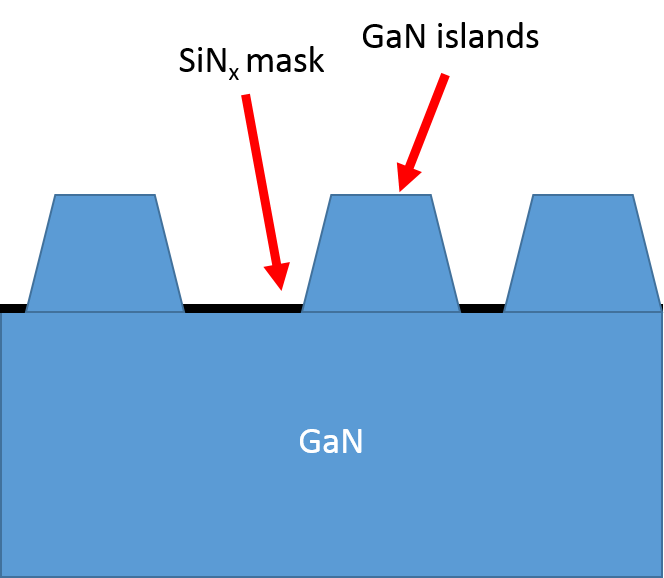
\includegraphics[width=1\linewidth]{Figs/Ch6/3D}
		\caption{}
		
	\end{subfigure}%
	\hspace*{0.6cm}
	\begin{subfigure}[b]{0.48\textwidth}
		\centering
		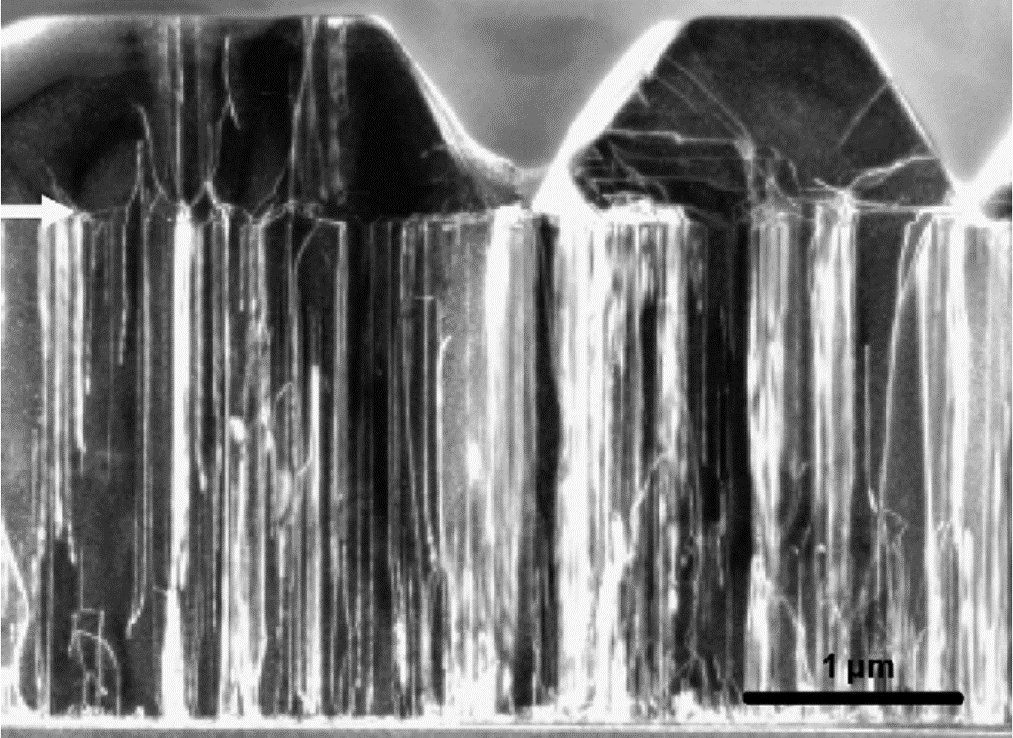
\includegraphics[width=1\linewidth]{Figs/Ch6/3D2}
		\caption{}
	\end{subfigure}%
	
	\caption{a) Schematic of $\mathrm{SiN_{x}}$ induced 3D growth and b) cross-sectional TEM image of an $\mathrm{SiN_{x}}$ interlayer (white arrow) on a GaN layer with GaN islands grown through the holes in the $\mathrm{SiN_{x}}$ layer. Adapted from \cite{Kappers2007}. Note that the $\mathrm{SiN_{x}}$ layer thickness is not to scale here, and has been expanded for the sake of clarity.}
	\label{3Dgrowth}
\end{figure}
\FloatBarrier

Tessarek \textit{et al.} suggest that the formation of the $\mathrm{SiN_{x}}$ layer on the non-polar facets of microrods is due to the presence of a Ga-droplet located at the top of the GaN rods during growth \cite{Tessarek2014a}. The Ga-droplet transforms into GaN due to the ammonia supply during post-growth cool down, and as such is only observable if the ammonia supply is interrupted during cool down. This droplet is highly attractive for Ga atoms in the gas phase and on the sidewalls of the microrod during growth, whilst Si and N atoms experience less adsorbance in this droplet due to their low solubility in liquid Ga \cite{Unland2003,Schmidt2010} thus resulting in a higher concentration of Si and N atoms on the microrod sidewall surfaces during growth. Following the growth of the microrod core during which silane is supplied ( see section \ref{nanorod growth}), ammonia is supplied continuously as the growth temperature is ramped down for QW growth temperature, thus resulting in the formation of the $\mathrm{SiN_{x}}$ layer. This combination of silane and ammonia is typically used to grow $\mathrm{SiN_{x}}$ on GaN \cite{Bottcher2003}. We expect the $\mathrm{SiN_{x}}$ coverage to be greater at the bottom of the rod, which experiences a longer silane exposure time during the growth process.

\begin{figure}[!h]
	\centering
	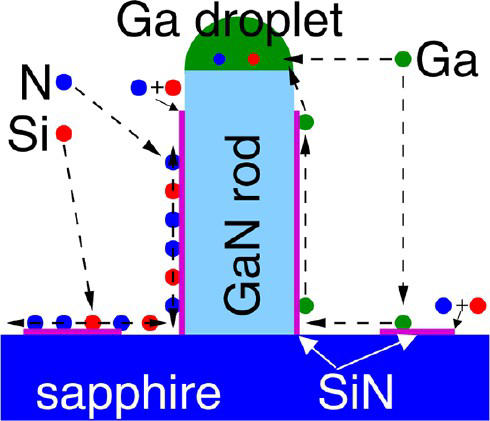
\includegraphics[width=0.7\textwidth]{Figs/Ch6/TessarekSi.jpg}
	\caption{Schematic of the $\mathrm{SiN_{x}}$ layer formation process: Si and N atoms experience low solubility in the Ga-droplet at the top of the rod and are thus present in greater concentration on the sidewall facets of the microrod. Reproduced from \cite{Tessarek2014a}.}
	\label{TessSi}
\end{figure}
\FloatBarrier     
In the context of the rods studied in this work, it is crucial to relate the Si content detected in the STEM-EDX experiments to the  $\mathrm{SiN_{x}}$ layer coverage. Reduced $\mathrm{SiN_{x}}$ coverage resulting either from a lower silane concentration or a lower exposure time \cite{Xie2007,Halidou2004} will lead to smoother surfaces as a result of complete GaN island overgrowth and coalescence prior to the growth of the InGaN QW stack. Xie \textit{et al.} reported incomplete coalescence of an overgrown GaN layer on a $\mathrm{SiN_{x}}$ layer for $\mathrm{SiN_{x}}$ deposition times exceeding 360 seconds \cite{Xie2007} even following a GaN overgrowth thickness of 4.5 $\mathrm{\mu m}$. As such, we expect the coverage of the $\mathrm{SiN_{x}}$ layer on the non-polar facets of the rods can heavily influence the subsequent growth of the InGaN QW stack and thus the optical properties of the rod. Indeed, in areas at the bottom of rods from sample A which show low emission in the CL we note the presence of voids, which are likely to result from the incomplete lateral coalescence of islands grown from the $\mathrm{SiN_{x}}$ layer such as the feature shown in Fig.\ref{A34}.b. Indeed, the presence of voids has been reported in epitaxial layer overgrowth (ELOG) of GaN, where a mask is intentionally used to induce 3D growth in order to reduce dislocation densities, as shown in Fig.\ref{ELOGvoids} \cite{Bennett2010,Ji2016}.

\begin{figure}[!h]
	\centering
	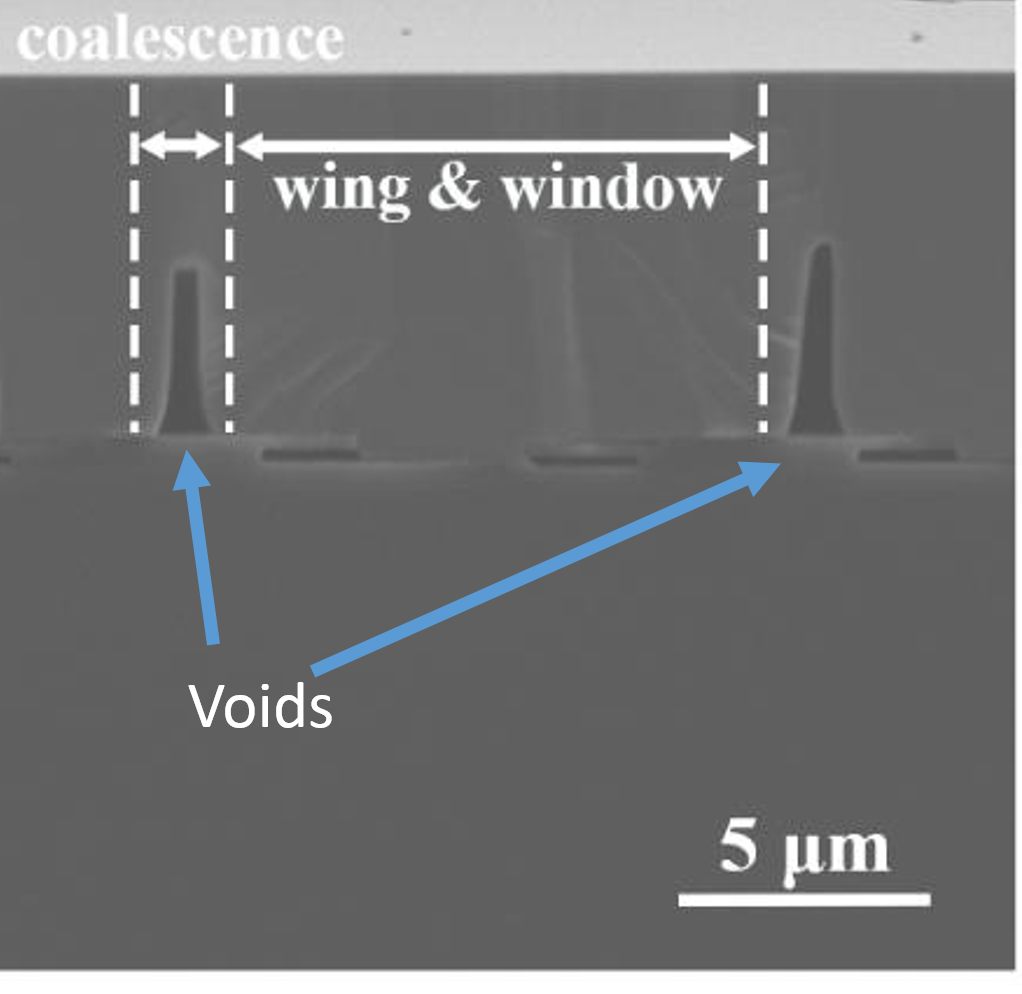
\includegraphics[width=0.7\textwidth]{Figs/Ch6/voidsELOG}
	\caption{Cross-sectional SEM image showing voids formed during ELOG of GaN. Adapted from \cite{Ji2016}. In the context of ELOG, 'wing' and 'window' describe sections of the epilayer grown laterally over the mask and from the holes in the mask respectively.}
	\label{ELOGvoids}
\end{figure}
\FloatBarrier 

Thus, though the use of silane is helpful in enhancing the vertical growth of the rods, the exposure time and silane concentration must be tailored carefully in order to achieve optimal coalescence conditions and thus obtain a uniform QW stack morphology and smooth microrod surface to allow for uniform emission over the length of the rod, a property desirable for applications such as LEDs and lasers. It is also important to note that the 'roughening' property of the $\mathrm{SiN_{x}}$ on the subsequent growth of III-nitride epitaxial layers is in some cases desirable, specifically in the growth of confined nanostructures such as QDs. As previously discussed, the use of nanomasks to grow III-nitride QDs \cite{Tanaka1996,Tu2004,Te-Chung2006} has been thoroughly investigated in \textit{c}-plane growth. As such, for applications such as single photon sources where QDs are required, the silane flow during the growth of the microrods may be tailored to encourage roughening of the subsequent InGaN active region in an attempt to grow non-polar QDs on the sidewall facets of the microrods. 


\section{Summary}

In this section we have examined the effect of Si on the morphology and optical properties of GaN/InGaN core-shell rods. Using SEM-CL we have shown the optical properties of the rods are heavily dependent on the silane concentration and exposure time during the rod growth, as reduced silane concentration and exposure time resulted in a more homogeneously emitting rod. By performing STEM-HAADF imaging on cross-sectional TEM lamellae prepared from the rods we correlated poorly emitting regions in the CL with regions containing a large amount of defects such as stacking faults and voids, as well as poor surface morphology. Following this we performed STEM-EDX on axial cross-sections prepared from the top and bottom regions of the rods, demonstrating a higher Si content detected in the $\mathrm{SiN_{x}}$ layer of the rods in regions with poor morphology, high defect densities and poor CL emission. We have also related the detected Si content of the $\mathrm{SiN_{x}}$ to the porosity of this layer, which heavily influences the subsequent overgrowth and coalescence of the GaN/InGaN active region. As such, we have determined that although the use of silane during rod growth is important to enhance growth in the vertical direction, it is also crucial to keep the silane concentration and exposure time as low as possible in order to maintain uniform microrod morphology and optical properties.


\section{Future Work}
We have used axial cross-section lift out methods to examine the effect of $\mathrm{SiN_{x}}$ coverage on microrod structure and emission. In the future, we may use correlated CL - radial cross-section TEM measurements to establish the structural cause of specific features in the emission such the blue shift of the QW emission going along the rod shown in Fig.\ref{sampleBscanCL}.
It is also valuable to attempt to tune the silane concentration and flow to maximise the length of the rod whilst maintaining good optical and structural properties. Halting the growth of the rods early may be useful in examining the manner in which $\mathrm{SiN_{x}}$ induces 3D growth on the non-polar facets of the rod, as well as the manner in which growth parameters may affect the subsequent coalescence of the 3D islands grown from the $\mathrm{SiN_{x}}$ mask.
In terms of further exploring the optical properties of the microrods, temperature dependent micro-PL experiments may be useful in determining the internal quantum efficiency of rods grown under different conditions. The presence of WGMs has been reported in III-nitride microrods \cite{Tessarek2014},  as such it may also be of interest to examine homogeneously emitting rods for WGM based lasing.
